\documentclass[journal]{IEEEtran}
\usepackage{color}
\usepackage[keeplastbox]{flushend}
\usepackage{subfigure}
\usepackage{multirow}
\usepackage{graphicx}
\bibliographystyle{IEEEtran}
% Some very useful LaTeX packages include:
% (uncomment the ones you want to load)
\usepackage{booktabs}
%% The amssymb package provides various useful mathematical symbols
\usepackage{booktabs}
\usepackage{threeparttable}
\usepackage{amsmath} 
\usepackage{amssymb}
\usepackage{latexsym}
\usepackage{flushend}
\usepackage{balance}
\usepackage{color}
\usepackage{subfigure}
\usepackage[colorlinks, 
           linkcolor=red,                     anchorcolor=blue,            
           citecolor=green ]{hyperref}
\linespread{1} 
\usepackage{caption}
\usepackage{url}
\usepackage{xcolor}
\definecolor{newcolor}{rgb}{.8,.349,.1}
% *** MISC UTILITY PACKAGES ***
%
\usepackage{ifpdf}

\usepackage{cite}
\usepackage{flushend}
%
\ifCLASSINFOpdf

\else

\fi

\hyphenation{op-tical net-works semi-conduc-tor}
\DeclareRobustCommand*{\IEEEauthorrefmark}[1]{%
    \raisebox{0pt}[0pt][0pt]{\textsuperscript{\footnotesize\ensuremath{#1}}}}
\usepackage{authblk} 
\begin{document}

\title{Underwater Image Enhancement with Lightweight Cascaded Network}



\author{Nanfeng Jiang,
        Weiling Chen,~\IEEEmembership{Member,~IEEE,}
        Yuting Lin,
        Tiesong Zhao,~\IEEEmembership{Senior Member,~IEEE,} and Chia-Wen Lin,~\IEEEmembership{Fellow,~IEEE}% <-this % stops a space
\thanks{This work is supported in part by the National Natural Science Foundation of China under Grants 62171134, 61901119 and in part by the Ministry of Science and Technology, Taiwan, under Grant MOST 110-2634-F-007-015. (*Corresponding author: Tiesong Zhao, t.zhao@fzu.edu.cn.)}

\thanks{N. Jiang, W. Chen and Y. Lin are with the Fujian Key Laboratory for Intelligent Processing and Wireless Transmission of Media Information, College of Physics and Information Engineering, Fuzhou University, Fuzhou 350108, China. (emails: \{201110003, weiling.chen, N181120063\}@fzu.edu.cn)}% <-this % stops a space

\thanks{T. Zhao is with the Fujian Key Laboratory for Intelligent Processing and Wireless Transmission of Media Information, College of Physics and Information Engineering, Fuzhou University, Fuzhou 350108, China, and also with the Peng Cheng Laboratory, Shenzhen 518055, China (e-mail: t.zhao@fzu.edu.cn)}

\thanks{C.-W. Lin is with the Department of Electrical Engineering, National
Tsing Hua University, Hsinchu 30013, Taiwan, and also with the
Institute of Communications Engineering, National Tsing Hua University, Hsinchu 30013, Taiwan (email: cwlin@ee.nthu.edu.tw)}}% <-this % stops a space




\markboth{IEEE transactions on Multimedia  }%
{Shell \MakeLowercase{\textit{et al.}}: Bare Demo of IEEEtran.cls for IEEE Journals}





% make the title area
\maketitle

% As a general rule, do not put math, special symbols or citations
% in the abstract or keywords.
\begin{abstract}
Due to light scatter and absorption in waterbody, underwater imaging can be easily impaired with low contrast and visual distortion. The resulting images are often unable to meet the quality requirements of human perception and computer processing. Therefore, Underwater Image Enhancement (UIE) has been attracting extensive research efforts. Although deep learning has demonstrated its great success in many vision tasks, its huge amounts of parameters and computations are not conducive to UIE in resource-limited scenarios. In this paper, we address this issue by proposing a Lightweight Cascaded Network (LCNet) based on Laplacian image pyramids. At each pyramid level, we implement cascaded blocks upon a residual network. Specifically, high quality residuals can be progressively predicted with significantly reduced complexity in a coarse-to-fine fashion. Furthermore, these sub-networks are recursively nested to build our LCNet, thereby reducing the overall computational complexity with reused parameters. Extensive experiments demonstrate that the proposed method performs favorably against the state-of-the-arts in terms of visual quality, model parameters and complexity.
\end{abstract}


% Note that keywords are not normally used for peerreview papers.
\begin{IEEEkeywords}
Underwater images, Image enhancement, Oceanic image processing.
\end{IEEEkeywords}






\IEEEpeerreviewmaketitle


\section{Introducation}
\begin{figure}[ht]
\centering 
{   
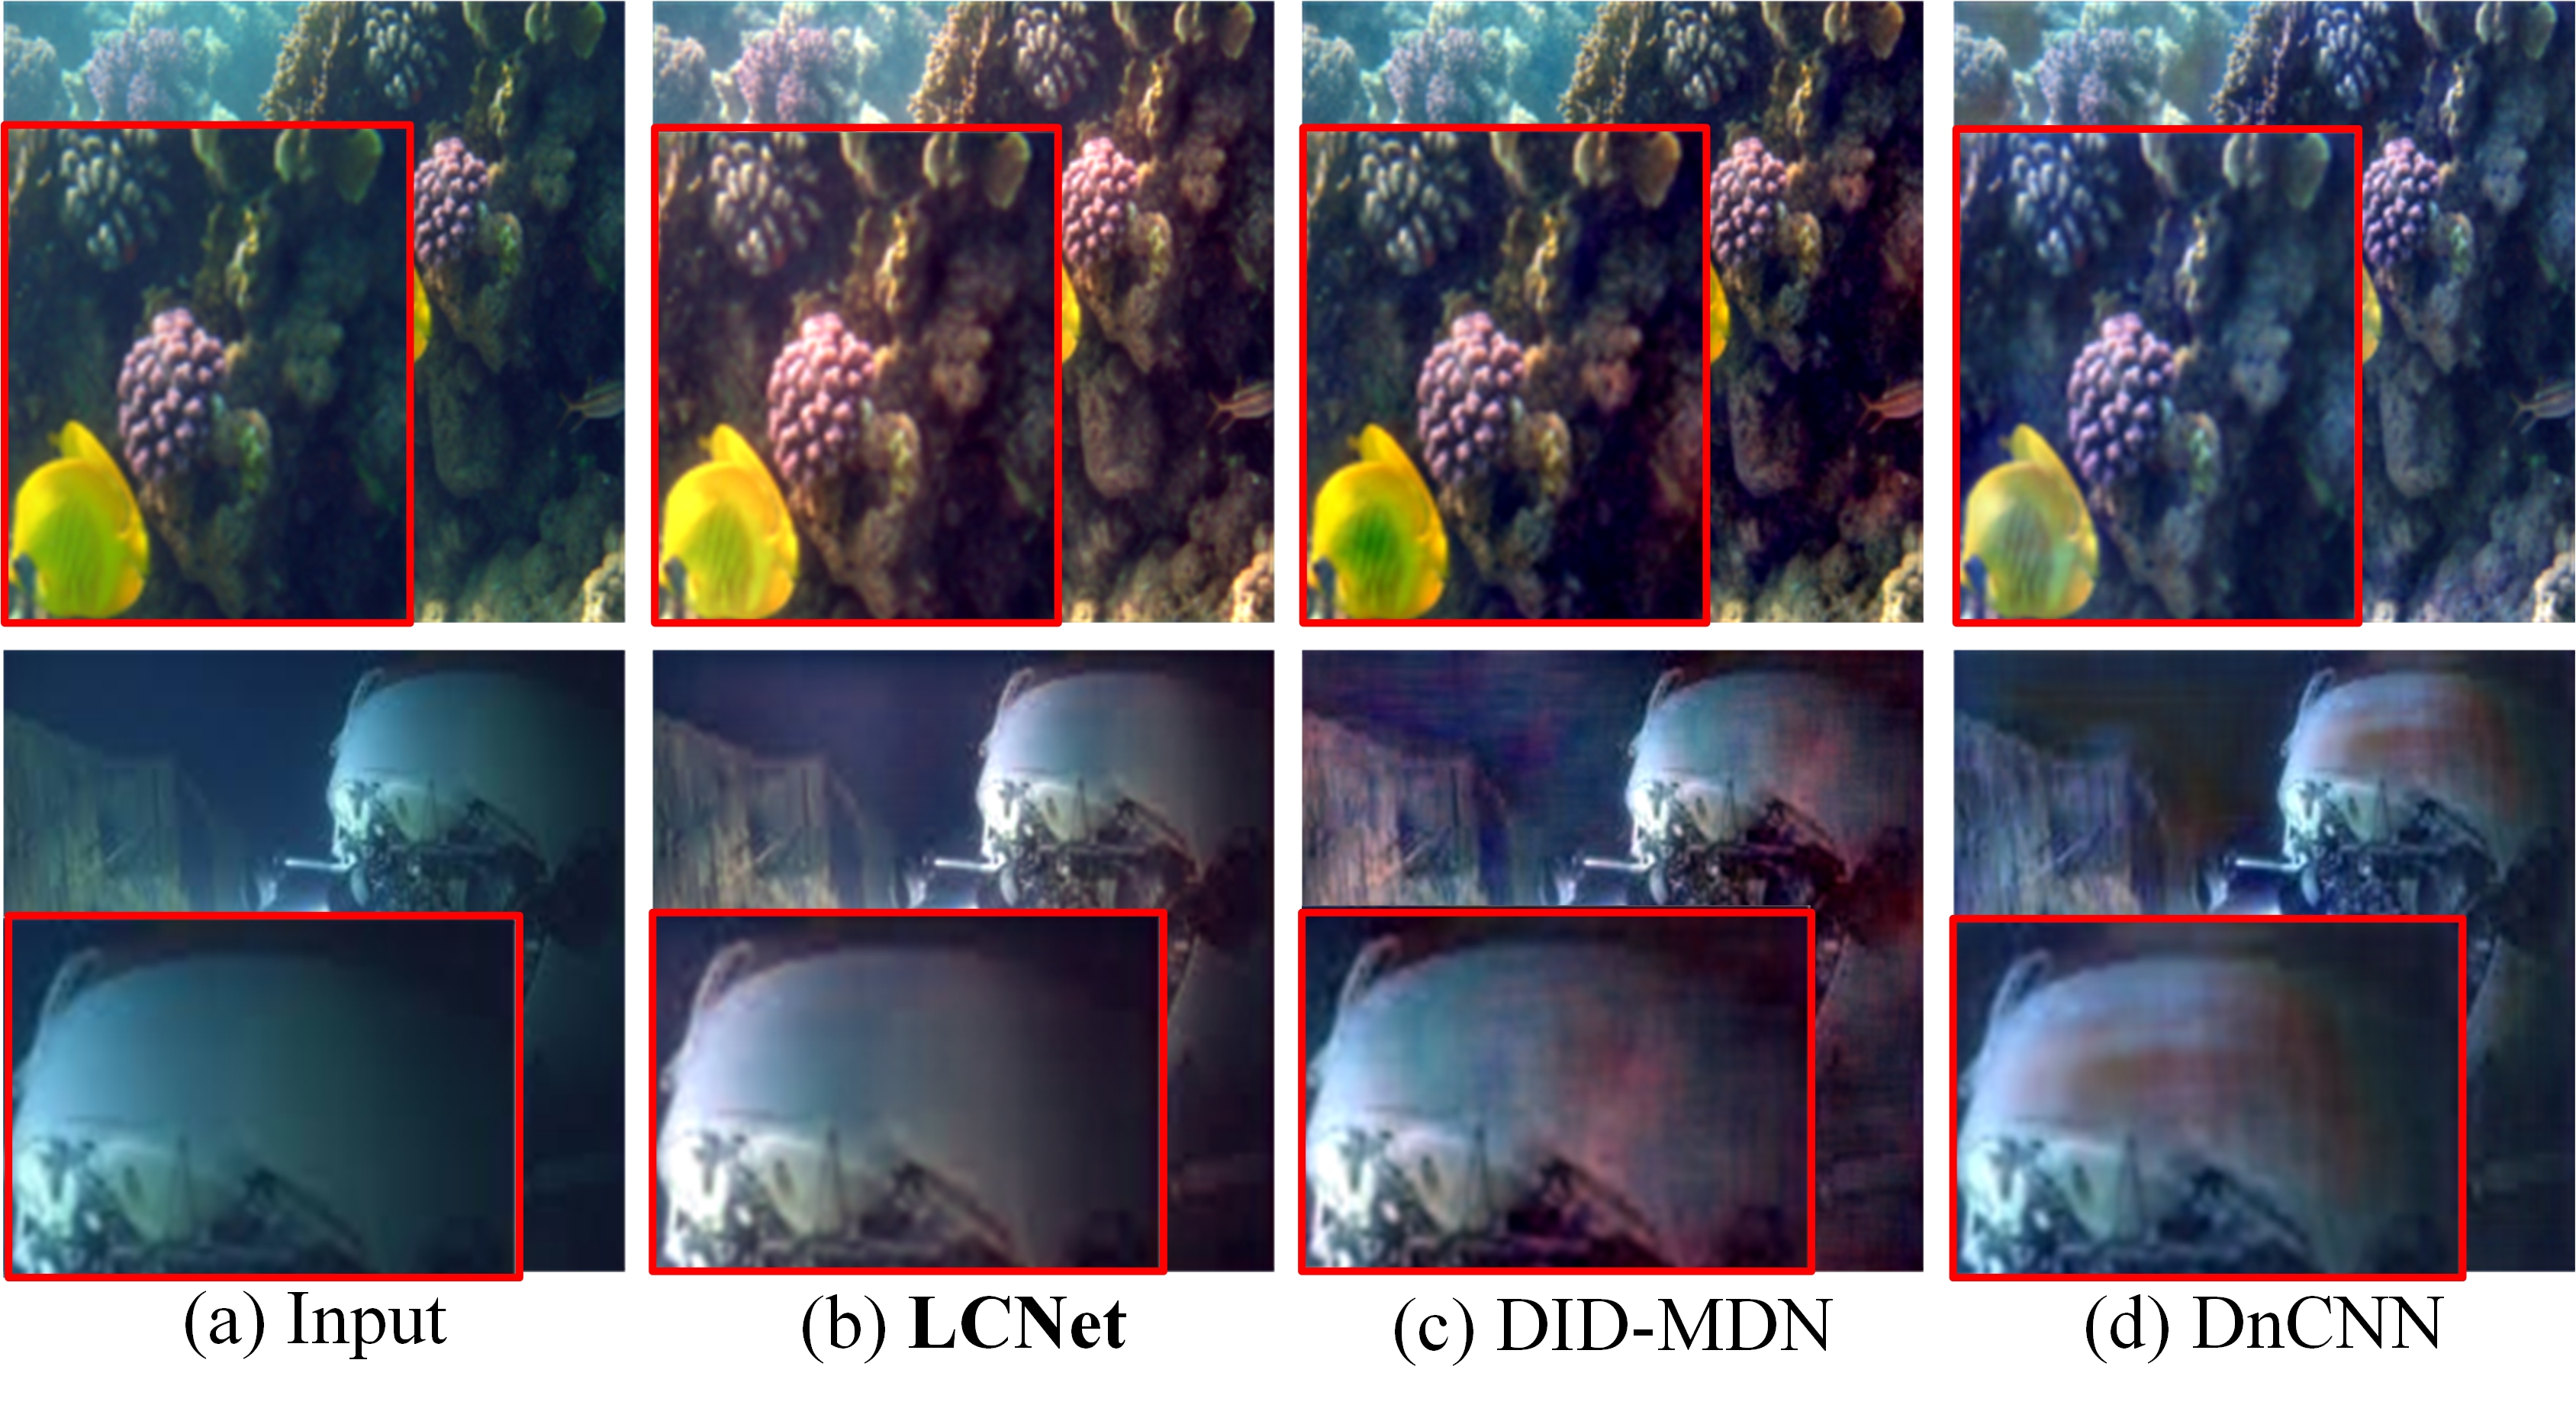
\includegraphics[width=0.5\textwidth]{Figs/Fig1.jpg}

}     
\caption{Examples of UIE tasks. (a) The raw underwater images, (b)-(d) enhanced results by our model, the
popular deraining method DID-MDN and denoising method DnCNN.}
\label{Fig1}
\end{figure}
Underwater Image Enhancement (UIE) is an important low-level image manipulation technique in oceanic tasks. Owing to light scattering, absorption effects and color variations, underwater images often suffer from quality degeneration, as shown in Fig. \ref{Fig1}-(a). These distorted or blurred images might become an obstacle of computer vision tasks, such as autonomous navigation \cite{lee2012vision}, vehicle tracking \cite{liu2016fully} and marine environmental surveillance \cite{underwaterscene}. In such case, visual enhancement of distorted images are essential to research in ocean environment. UIE techniques are thereby required to facilitate these tasks. It can be observed from Fig. \ref{Fig1}-(b) that the images after UIE are with enhanced visual quality, which may help succeeding image processing or vision tasks. 


In the past decade, visual restoration and enhancement algorithms have been benefited from large-scale training data and deep Convolutional Neural Networks (CNNs). These methods include deraining \cite{DID-MDN,zhang2019image,wang2020deep}, dehazing \cite{dehazeli2018single,liuICCV2019GridDehazeNet,yang2019single}, denoising \cite{zhang2017beyond}, \textit{etc.} 
However, UIE is different from these popular low-level tasks such as denoising/deraining in the following aspects. First, underwater images present different types of visual appearances. In popular denoising problems, distortions are generated by additional noises or unwanted objects; while in UIE, distortions are generated by underwater imaging under unsatisfactory lighting conditions. As a result, we can still observe original scenes covered by additional noises; however, this does not work well for underwater scenes with visual range and contrast loss. Second, assessing UIE images require different quality evaluation metrics. It is well known that in visual quality assessment, collecting the original references of the restored/enhanced images is a critical issue. With the high difficulty to recover an original reference for an underwater image, the quality assessment of UIE images differs from that of conventional images. Therefore, popular UIE quality metrics, such as Underwater Color Image Quality Evaluation (UCIQE) \cite{yang2015underwater} and Underwater Image Quality Measure (UIQM) \cite{panetta2015human}, are specially designed for underwater images. Third, due to the above differences, existing denoising/deraining methods show inferior performances for the UIE task. An example is shown in Fig. \ref{Fig1}, where the denoising method DnCNN \cite{zhang2017beyond} generates color cast artifacts while the deraining method DID-MDN \cite{DID-MDN} generates over-saturation. As a result, there is still a need to develop effective UIE algorithms.

Until now, typical UIE algorithms have been developed based on statistical models. The methods proposed in \cite{carlevaris2010initial,chiang2011underwater,Wen2013Single} improve visual quality or calibrate color casts by combining traditional enhancement models with latent parameter estimation. Recently, deep CNNs have shown their strengths in image restoration. In these algorithms, large-sized parameters and memory footprints are usually required to construct complicated network layers and stages. However, self-guiding and self-powered marine vehicles, such as Autonomous Underwater Vehicles (AUVs) and Remotely Operated Vehicles (ROVs), are usually with limited computing power and storage that are not sufficient to support comprehensive computing locally. On the other hand, an Underwater Acoustic Channel (UAC) is also known to offer too poor-quality communication to support cloud-based image processing. In this case, existing methods are often not applicable owing to their heavy computational requirements. 

To bridge the gap between existing UIE approaches and real-world applications, we exploit the potential of lightweight network that benefits both effectiveness and efficiency for the UIE task. Recently, many low-level tasks (\textit{e.g.,} LapSRN \cite{lai2018fast} for single image super-resolution, LPNet \cite{fu2019lightweight} for single image rain removal) use Laplacian pyramid to build their lightweight architecture and achieve promising results. Motivated by them, we inherit the advantages of Laplacian Pyramid and propose a Lightweight Cascaded Network (LCNet) to enhance underwater images effectively and efficiently. LCNet is an enhanced version of LPNet \cite{fu2019lightweight} with the following improvements. First, LCNet takes all-rounded advantages of the correlated information across different scales. Second, at each pyramid level, we build a cascaded sub-network based on several recursive blocks, which can make full use of the hierarchical features via global connections. Third, in each block, we conduct residual learning in a recursive manner to improve performance with reused model parameters.

In summary, the major contributions of this paper are as follows:
\begin{itemize}
\item We propose an LCNet to alleviate undesired underwater color degradation and reduce the network parameters through image pyramids and parameters reuse. Besides, this model is able to learn complicate feature maps at different scales and improve model robustness.


 
\item At each pyramid level, we design a cascaded sub-network, which effectively handles different types of underwater images with a recursive strategy and a coarse-to-fine image residual estimation. We also introduce perceptual loss to constrain the network training.


\item The proposed model achieves an excellent balance among visual quality, inference speed, model parameters and complexity. As demonstrated by extensive experiments, it could benefit the object detection in underwater environment.
\end{itemize}



\section{Related Work}
Existing UIE methods can be classified into three categories:
non-physics model-based, physics model-based and deep
learning-based methods. 
\subsection{Non-physics Model-Based Methods}
Non-physics model-based methods adjust pixel values to improve image quality without modeling mathematical formulations \cite{iqbal2010enhancing,ghani2015underwater,fusion-based,fu2017two,fu2014retinex,zhang2017underwater}. In \cite{iqbal2010enhancing}, Iqbal \textit{et al}. designed a contrast correction model to remove the bluish and red color. Ahmad \textit{et al}. \cite{ghani2015underwater} followed the Rayleigh distribution within certain range to remove extra artifacts. Ancuti \textit{et al}. \cite{fusion-based} proposed a UIE solution built on the multi-scale fusion principle. After that, Ancuti \textit{et al}. \cite{ancuti2017color} also introduced a novel approach to remove the haze in underwater, improving the visual performance. Ancuti \textit{et al.} \cite{ancuti2016multi} designed a UIE approach that estimates the back-scattered light locally. Recently, Ancuti \textit{et al}. \cite{ancuti2019color} proposed a Color Channel Compensation (3C) approach, which effectively enhances in terms of color appearance. Fu \textit{et al}. \cite{fu2017two} proposed a two-step UIE procedure,  including a color correction and a contrast enhancement. Moreover, several works  \cite{fu2014retinex,zhang2017underwater} of UIE were based on retinex theory, Fu \textit{et al}. \cite{fu2014retinex} proposed a variational framework to decompose the reflectance and illumination, which are utilized in further enhancement. Zhang \textit{et al}. \cite{zhang2017underwater} proposed an extended multi-scale retinex-based UIE method, which processed the underwater images in CIELAB color space. These methods perform well, but suffer from low contrast, detail loss and color deviations due to the complexity of underwater environment and limited observations \cite{liu2020real}.
\begin{figure*}[h] 
\centering 
{   
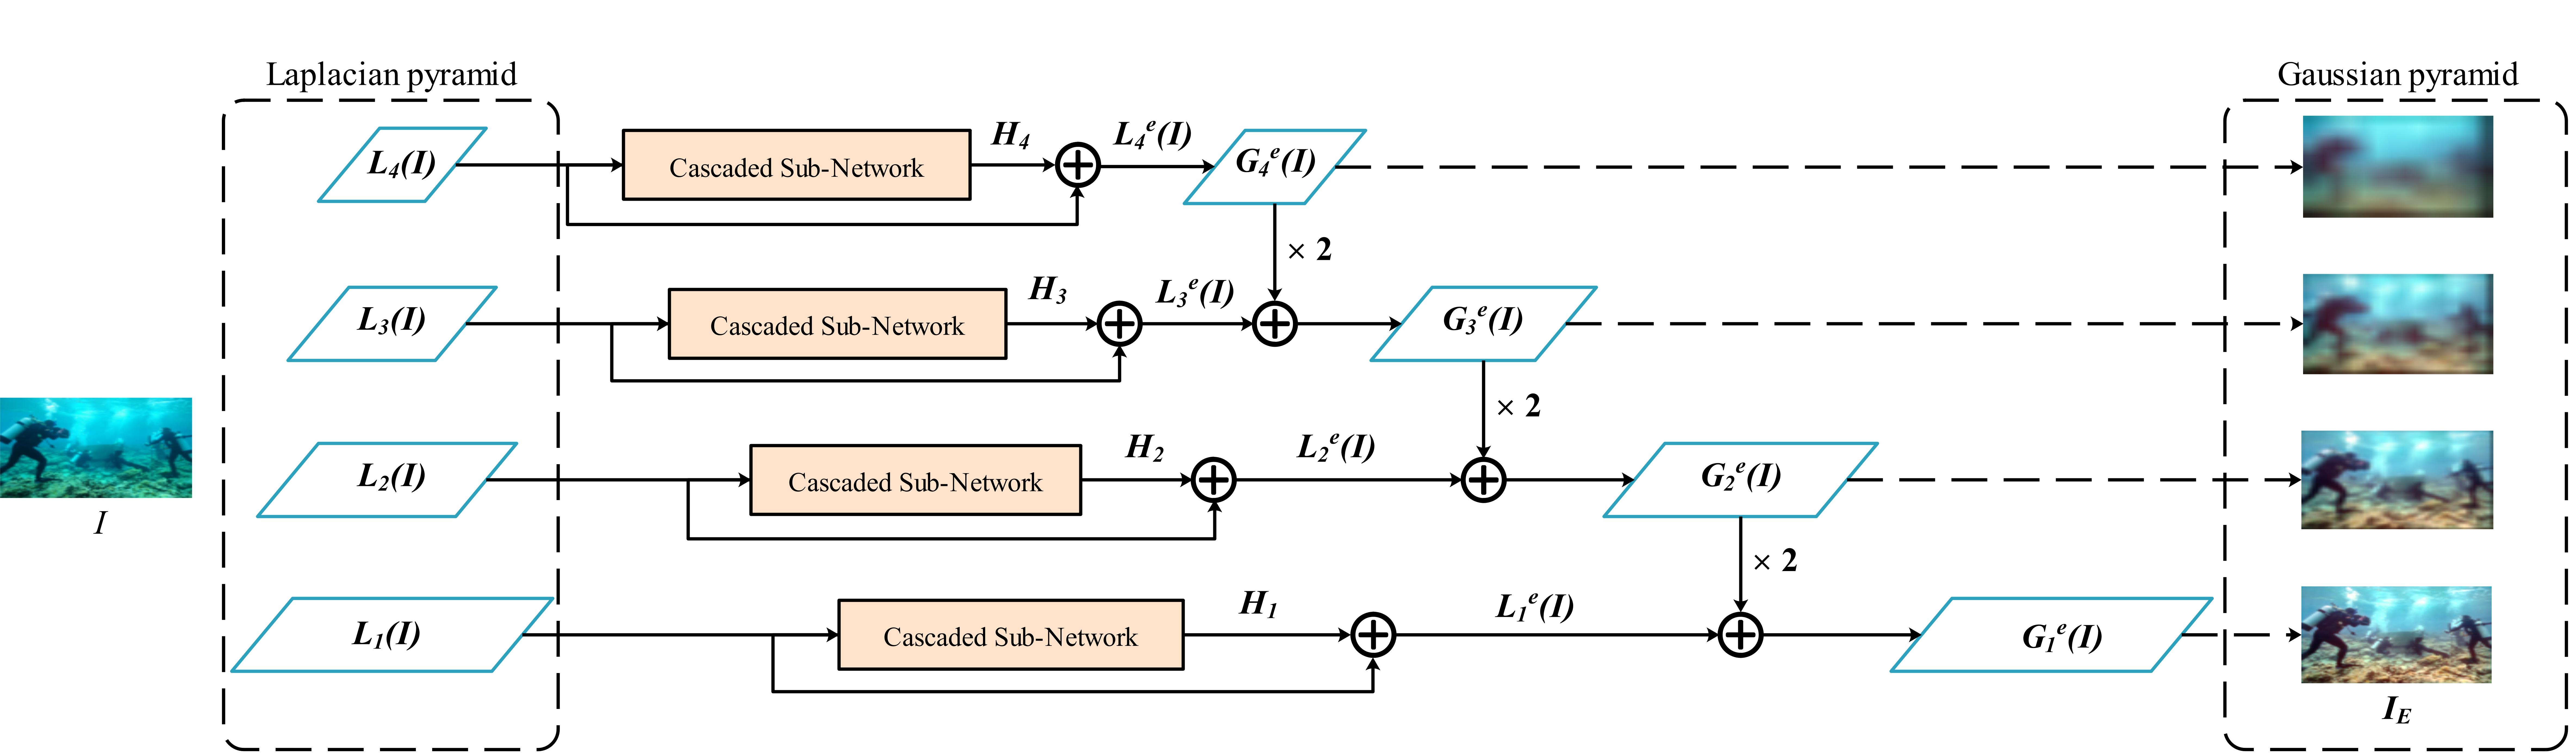
\includegraphics[width=0.9\textwidth]{Figs/Fig2.png}
}          
\caption{Architecture of the proposed LCNet. It achieves multi-scale image enhancement with three steps:
pyramid decomposition, multi-scale enhancement and image
reconstruction.}
\label{Fig2} 
\end{figure*} 
\subsection{Physics Model-Based Methods}
Instead of pixel-to-pixel mapping, the physics model-based methods explicitly characterize the physical imaging process, and estimate the imaging parameters from observations and various prior assumptions\cite{he2010single,chiang2011underwater,UDCP,GDCP,Histogram-prior,akkaynak2019sea,serikawa2014underwater}.
Chiang \textit{et al}. \cite{chiang2011underwater} proposed to enhance underwater images by combing the Dark Channel Prior (DCP) \cite{he2010single} with wavelength-dependent compensation algorithm. In \cite{UDCP}, an Underwater DCP (UDCP) was proposed based on the
fact that the information of red channel is undependable in an underwater image. Peng \textit{et al}. \cite{GDCP} proposed a Generalized DCP (GDCP) that estimated ambient light using the depth-dependent color change. Recently, Berman \textit{et al.} \cite{berman2020underwater} proposed a method to recover the distance maps and object colors in scenes taken under water and under ambient illumination. In addition, Li \textit{et al}. \cite{Histogram-prior} proposed to combine an underwater image dehazing model with contrast enhancement. More recently, Akkaynak \textit{et al}. \cite{akkaynak2019sea} designed an underwater image color correction method based on a physically accurate model. In summary, the non-physics and physics model-based methods depended on various observations and prior assumptions.
 Therefore, these algorithms cannot be well generalized to some specific scenes \cite{GDCP}.

\subsection{Deep Learning-Based Methods}
Very recently, deep CNNs have promoted the development
of computer vision and image processing \cite{8100962,8820082,li2020asif,zheng2020scale,li2018deep,liu2019theoretically,dehazeli2018single,fu2017removing,Zero-DCE++}. 
As for the UIE, deep learning-based methods also
led to a fast development and achieved state-of-the-art performance \cite{uwcnn,dense-gan,li2017watergan,water-net,water-gan,lu2018low}. In \cite{li2017watergan}, Li \textit{et al}. employed the Generative Adversarial Network (GAN) to build a WaterGAN model, which incorporated the process of underwater image formation to generate high resolution outputting images. Guo \textit{et al}. \cite{dense-gan} proposed a multi-scale Dense-GAN, which improves UIE by learning the distribution of ground truth images in the feature domain. Recently, Li \textit{et al}. \cite{li2021underwater} proposed a medium transmission-guided decoder network to enhance the response of our network
towards quality-degraded regions. For the diversity of underwater images, Li \textit{et al}. \cite{uwcnn} also proposed to train an end-to-end UWCNN network, which directly reconstructs the clear latent image based on 10 types of underwater images. Hou \textit{et al.} proposed an underwater residual network to jointly optimize transmission and correct color casts \cite{hou2018joint}. The authors of \cite{water-gan} proposed a Cycle-consistent Generative Adversarial Network (Cycle-GAN) for UIE. In \cite{water-net}, Li \textit{et al}. developed a real-world underwater image database of Underwater Image Enhancement Benchmark (UIEB), and proposed a CNN model (called Water-Net) trained by this dataset for UIE. Although most deep learning-based methods have delivered excellent performances, they are at the expense of high complexity. To address this issue, some lightweight methods have been applied in other low-level tasks. For example, Fu \textit{et al}. \cite{fu2019lightweight} introduced a Lightweight Pyramid Network (LPNet) for single image deraining. This network uses several sub-networks to predict the clean Gaussian pyramid, which simplifies the learning problem. LPNet requires fewer than 8K parameters while still achieving promising performance.


\section{Proposed Method}
As discussed above, a practical UIE method should be capable of effectively processing underwater images with low complexity. In this work, it is achieved by multi-scale processing and recursive networks. Detailed illustration of our model is presented as follows.
\subsection{Philosophy of Model Design}
Underwater images have their particular features which impede the further improvement of UIE performance. Due to various light conditions and water current, the color details of images might be blended with object edges and backgrounds, which makes the pixel-domain mapping into a difficult task. Moreover, the superior performance of a deep network usually requires an inevitable increase of model parameters, which make it costly in real-world application. To address these problems, we attempt to build a compact network by making full use of multi-scale features.

The introduction of multi-scale processing is also motivated by image quality assessment and other low-level tasks. In view of quality assessment, a user measures the quality of an image based on its multi-scale fidelities and textures \cite{wang2003multiscale}, which inspires us to enhance images at different scales. Moreover, the multi-scale processing has also been widely employed in low-level processing for its ability to decompose a difficult problem to several easier sub-problems. In this work, we achieve the multi-scale processing with three steps: pyramid decomposition, multi-scale enhancement and image reconstruction.

In multi-scale enhancement, we introduce a compact network with lightweight sub-networks to enhance images in a coarse-to-fine manner. After pyramid decomposition, we are able to design simple sub-networks to handle each pyramid level in a divide-and-conquer way, resulting in compact sub-networks and fast computation. In addition, we also design each sub-network with recursive residual networks, that allow parameter reuse to further benefit the lightweighting of our model.
 


\subsection{The Framework of LCNet}
Based on the above discussions, we propose LCNet, that consists of pyramid decomposition, multi-scale enhancement and enhanced image reconstruction. LCNet is a pyramid network that incorporates a series of lightweight sub-networks to progressively refine the image details for output. The general architecture of LCNet is illustrated in Fig. \ref{Fig2}. We first decompose an underwater image \(I\) into a multi-level Laplacian pyramid. For each pyramid level, we build a sub-network to enhance image residuals. All sub-networks share the same architecture, but they are trained separately (\textit{i.e.}, no weight sharing). Finally, we enhance all Laplacian residuals at different levels and then reconstruct a Gaussian pyramid from coarse to fine to obtain the output enhanced image. Let \(I\) and \(I_{E}\) respectively denote an input underwater image and its enhanced version, the overall model can be expressed as
\begin{equation}
 I_{E}={\rm LCN}(I),
\end{equation}
where \(\rm{LCN(\cdot)}\) denotes the operation of LCNet, which is elaborated as follows.


\subsection{Pyramid Decomposition}
In this work, we employ Laplacian pyramid decomposition to decompose an image into multi-scale sub-bands. The Laplacian image pyramid is a mature algorithm with low computational cost \cite{lai2018fast}. Thanks to its multi-scale decomposition ability, the enhancement problem can be separately performed at different scales, thereby simplifying the learning process. In particular, the most time-consuming part of Laplacian decomposition can be realized by convolutions with GPU acceleration, thereby achieving significant speed-up. The multi-scale decomposition also facilitates the network to take advantage of sparsity at each level, thereby removing color artifacts \cite{iqbal2020underwater}.

As shown in Fig. \ref{Fig2}, we adopt Laplacian pyramid decomposition to generate a set of images \(L_{n}\) with \(N\) levels:
\begin{equation}
L_{n}\left ( I\right )=G_{n}\left ( I \right )-u\left ( G_{n+1}\left ( I\right )\right),
 \label{equation2} 
\end{equation}
where \(G_{n}(I)\) and \(\rm{u(\cdot)}\) are the \(n\)-th Gaussian pyramid image and an upsampling operator, respectively. \(L_{n}(I)\) is the \(n\)-th Lapcian pyramid image, which is constructed by taking the difference between \(G_{n}(I)\) and \(u(G_{n+1}(I)\)(\(n\) = 1, 2, ..., \(N\)-1). \(L_{N}(I)\) = \(G_{N}(I)\) and \(G_{1}(I)\) = \(I\).



\begin{figure*}[h] 
\centering 
{   
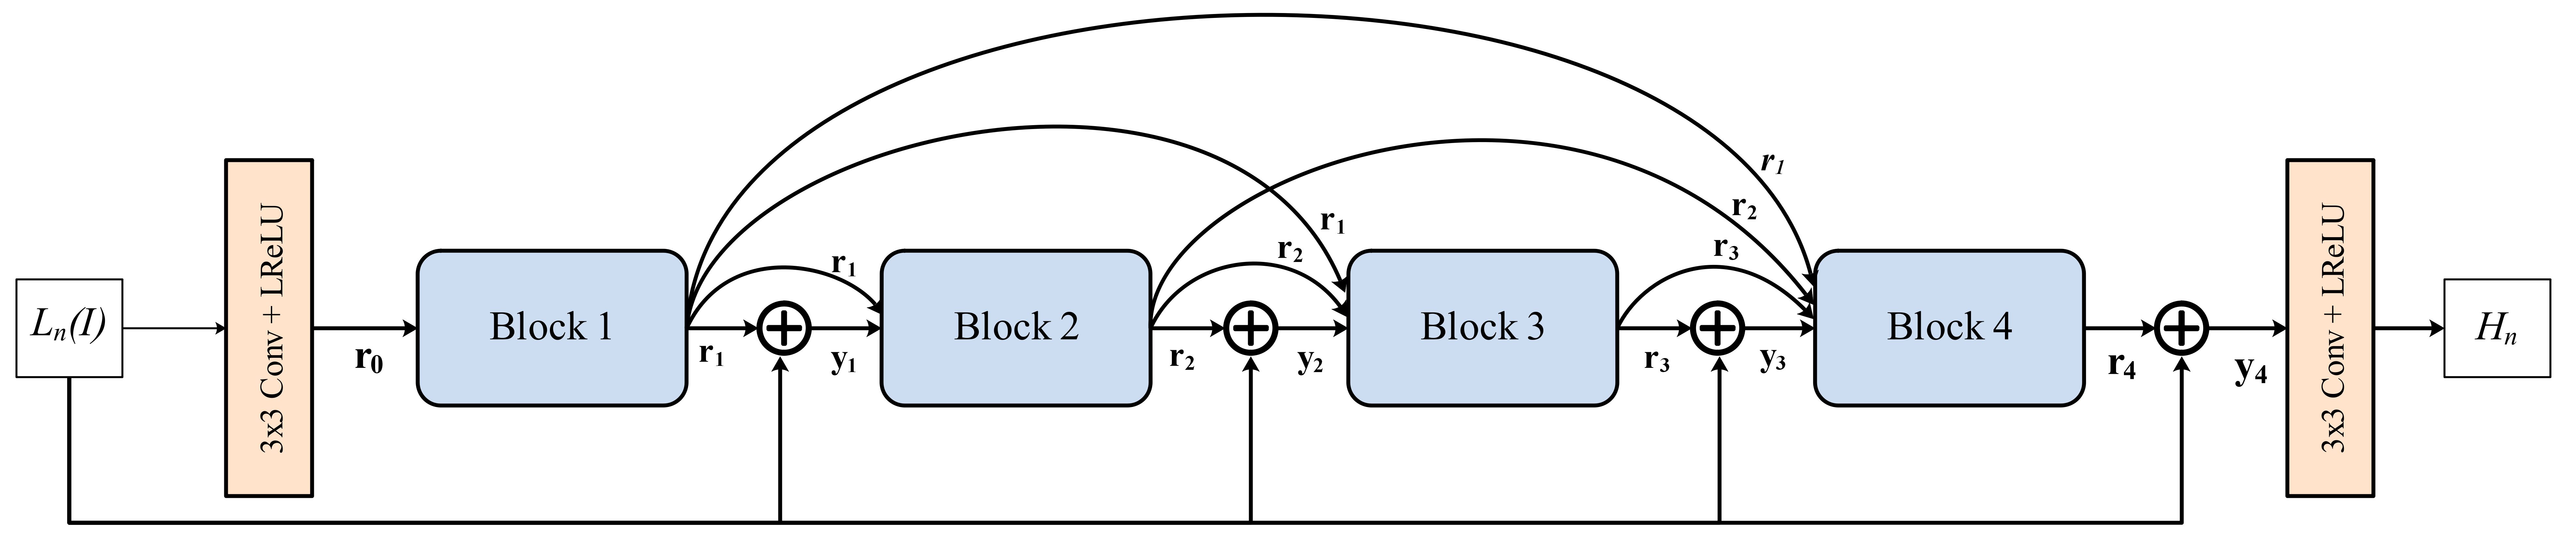
\includegraphics[width=0.95\textwidth]{Figs/Fig3.png}
}          
\caption{Architecture of cascaded sub-network, which is composed of four recursive blocks.}
\label{Fig3} 
\end{figure*} 

\begin{figure*}[h] 
\centering 
{   
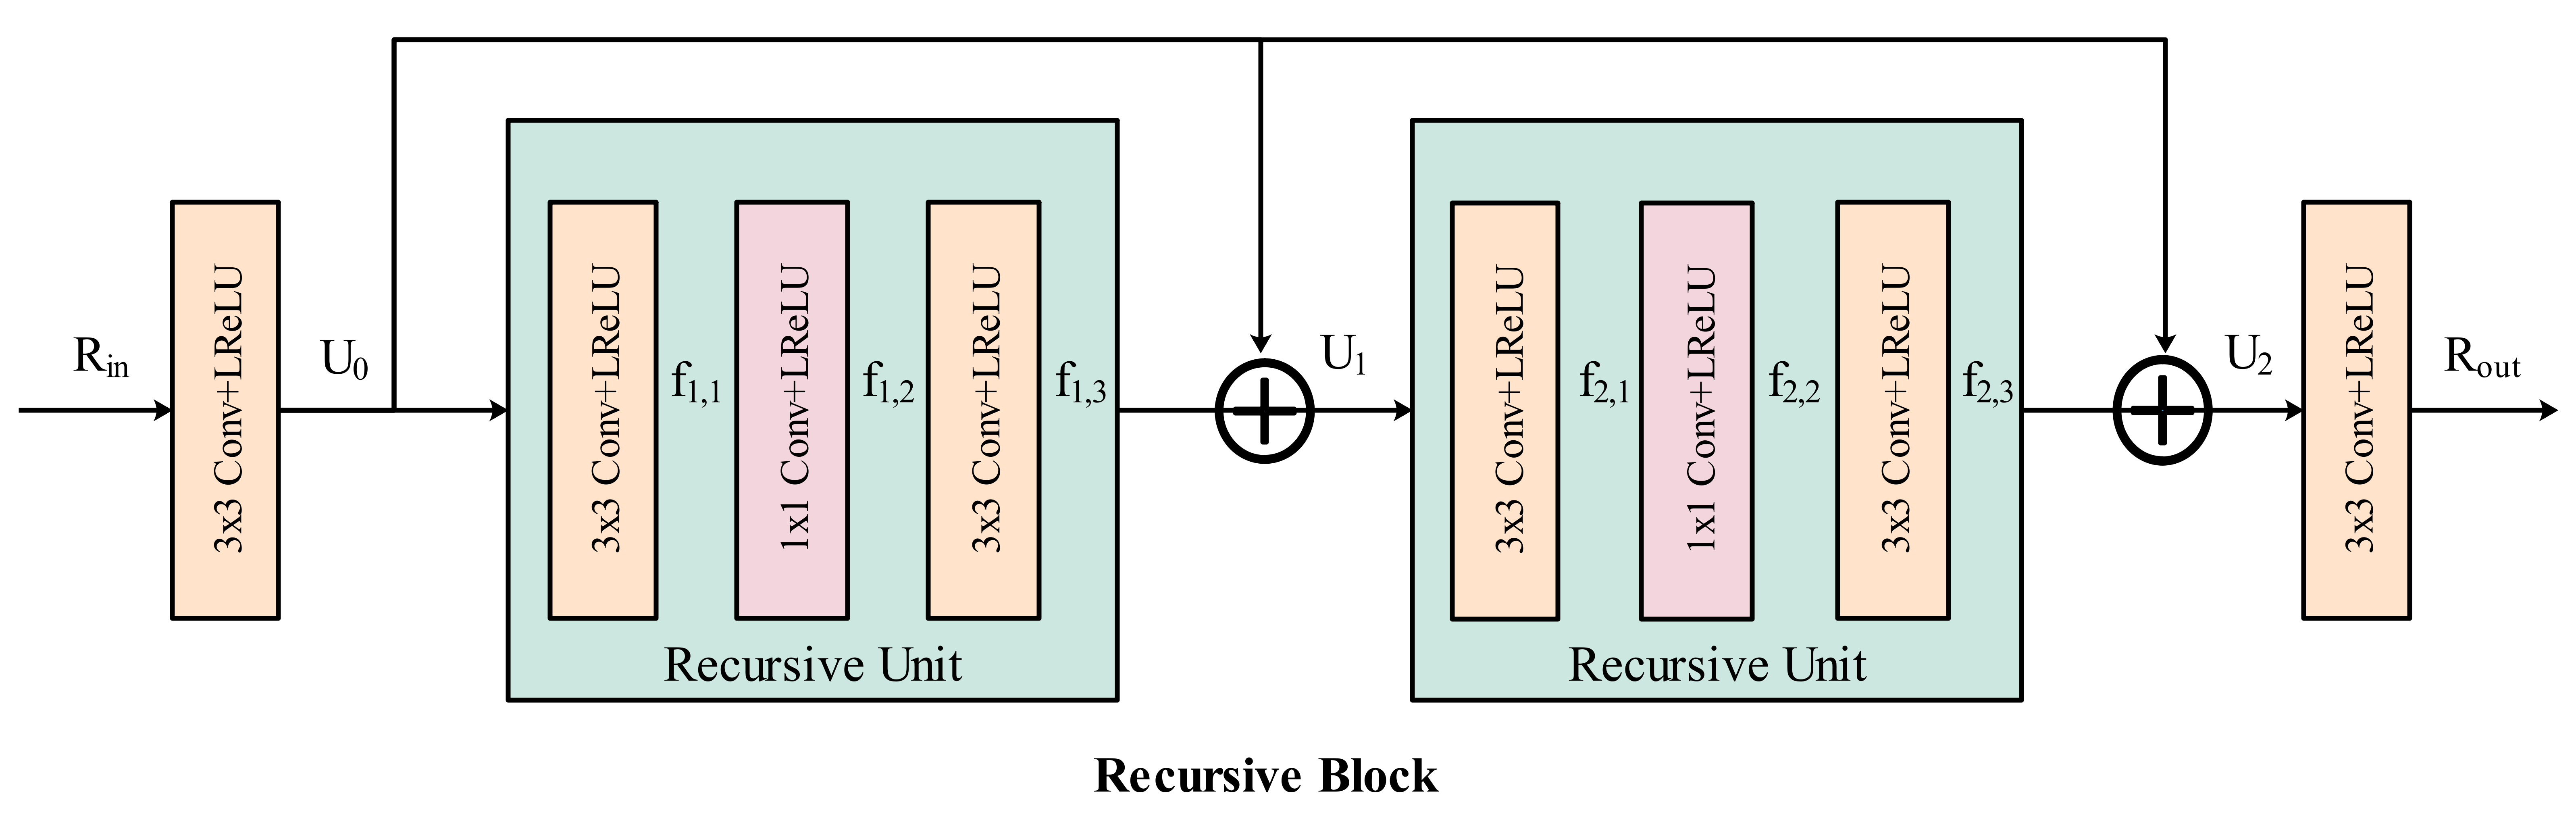
\includegraphics[width=0.9\textwidth]{Figs/Fig4.png}
}          
\caption{Architecture of recursive block, which is composed of two recursive units.}
\label{Fig4} 
\end{figure*} 

\subsection{Multi-scale Enhancement}
It is often desirable in practical applications to apply a lightweight network to trade model performance for efficiency. In this work, we realize it by an efficient model and parameter reuse across different pyramid levels. 

With Laplacian pyramid decomposition, we are able to design simple sub-networks to handle each pyramid level in a divide-and-conquer way, resulting in compact sub-networks and fast computation. In addition, we also design each sub-network in a recursive processing manner, which allows parameter reuse to further benefit the lightweighting of our model. The illustrations of multi-level processing are as follows:

After decomposing \(I\) into different pyramid levels, we build a set of sub-networks for enhancement. As shown in Fig. \ref{Fig3}, each sub-network consists of two 3 \(\times\) 3 convolutional layers and four blocks. At the front and end of sub-network, convolutional layers with Leaky Rectified Linear Units (LReLUs) \cite{xu2015empirical} are added to adapt to the feature dimensions. All sub-networks share the
same architecture but their parameters are separately trained. Thus, at each level, the sub-network
only needs to consider the input's own physical characteristics
(\textit{e.g.,} low or high frequencies). The basic formulation of sub-network at the \(n\)-th level can be expressed as
 \begin{equation}
 \begin{aligned}
 H_{n}=f_{C}(L_{n}(I)),\\
 \end{aligned}
\end{equation}
where \(f_{C}(\cdot)\) denotes the operation of sub-network, \(n\) = 1, 2, ..., \(N\).


\subsubsection{Cascaded Sub-Network}
The deep residual networks (ResNet) achieve fast and stable convergence that addresses the vanishing gradient problem in back propagation. By learning a residual mapping for a few stacked layers, deep neural networks can be easily trained with impressive performance. In contrast, Tong \textit{et al.} \cite{tong2017image} proposed to concatenate feature maps densely from shallower to deeper layers to alleviate the vanishing gradient problem and reduce the number of model parameters. It can be interpreted as there is no need to learn redundant features. Inspired by this, we perform a global residual learning with a shortcut in each block to facilitate the learning process.


As shown in Fig. \ref{Fig3}, Block 1 takes an input \(r_{0}\), which represents the features extracted from \(L_{n}(I)\), and generates an output \(r_{1}\) to its succeeding blocks. The combination of \(r_{1}\) and \(L_{n}(I)\) forms \(y_{1}\) as another input to the next block. Block 2 receives \(y_{1}\)and \(r_{1}\) and outputs \(r_{2}\), which serves as an input to all its succeeding blocks as well as \(y_{2}\). Sequentially, Blocks 3 and 4 also receive features from their preceding blocks and output features. In particular, the output of Block 4, denoted as \(r_{4}\), is utilized to generate \(y_{4}\) only, that is further processed by the convolutional layer to generate the enhanced residual \(H_{n}\). The above process can be expressed as
\begin{equation}
 \begin{aligned}
r_{0}&=c_{3 \times 3}(L_{n}(I)),\\
r_{1}&=f_{B_1}(r_{0}),\\
y_{1}&=r_{1}+L_{n}(I),\\
r_{2}&=f_{B_2}(y_{1},r_{1}),\\
y_{2}&=r_{2}+L_{n}(I),\\
r_{3}&=f_{B_3}(y_{2},r_{2},r_{1}),\\
y_{3}&=r_{3}+L_{n}(I),\\
r_{4}&=f_{B_4}(y_{3},r_{3},r_{2},r_{1}),\\
y_{4}&=r_{4}+L_{n}(I),\\
H_{n}&=c_{3 \times 3}(y_{4}),
\end{aligned}   
\end{equation}
where \(c_{3 \times 3}(\cdot)\) denotes the operation of convolutional layer with 3 \(\times \) 3 kernel, \(f_{B_b}(\cdot)\) denotes the operation of each block and \(r_{b}\) denotes the output of the \(b\)-th block within a sub-network, \(b\) = 1, 2, 3, 4. The output of Fig. \ref{Fig3} is then cascaded to fuse all information of sub-network. Through this procedure, the LCNet quickly predicts residuals from the shallower to deeper layers.


\subsubsection{Recursive Strategy}

In each pyramid level, we adopt a lightweight cascaded sub-network consisting of several blocks, where each block adopts convolutional layers and LReLUs to formulate a nonlinear mapping of features. As a result, the cascaded networks achieve feature extraction with a high model complexity. To develop a lightweight model, we adopt the recursive scheme in each block, in which two recursive units are deployed with shared weights that can be trained simultaneously. Through weight sharing, the model parameters are significantly reduced. As shown in Fig. \ref{Fig4}, each block has two convolutional layers and two recursive units. The processing within a block can be expressed as
\begin{equation}
 \begin{aligned}
U_{0}&=c_{3 \times 3 \times b}(R_{inb}),\\
U_{1}&=R(U_{0})+U_{0},\\
U_{2}&=R(U_{1})+U_{0},\\
R_{outb}&=c_{3 \times 3}(U_{2}),\\
\end{aligned}
\end{equation}
where \(R_{inb}\), \(R_{outb}\) are the input and output of the \(b\)-th block (\(b\) = 1, 2, 3, 4). \(R(\cdot)\) denotes the operation of the recursive unit, \(U_{t-1}\) and \(U_{t}\) are the input and output of the \(t\)-th unit (\(t\) = 1, 2). In particular, the \(c_{3 \times 3 \times b}\) is used for adapting to the different dimensions of \(R_{inb}\). The input-output relations within blocks can be expressed as
\begin{equation}
 \begin{aligned}
R_{in1}&=r_{0},\\
R_{out1}&=r_{1},\\
R_{in2}&=(r_{1},y_{1}),\\
R_{out2}&=r_{2},\\
R_{in3}&=(r_{1},r_{2},y_{2}),\\
R_{out3}&=r_{3},\\
R_{in4}&=(r_{1},r_{2},r_{3},y_{3}),\\
R_{out4}&=r_{4}.\\
\end{aligned}
\end{equation}
Each unit can be formulated as
\begin{equation}
\begin{aligned}
f_{t,1}&=c_{3 \times 3}(W_{t,1};U_{t-1}),\\
f_{t,2}&=c_{1 \times 1}(W_{t,2};f_{t,1}),\\
f_{t,3}&=c_{3 \times 3}(W_{t,3};f_{t,2}),\\
\end{aligned}
\end{equation}
where \(f_{t,1}\), \(f_{t,2}\) and \(f_{t,3}\) are intermediate features in corresponding \(t\)-th recursive unit, respectively. \(W_{t,1}\), \(W_{t,2}\) and \(W_{t,3}\) are weights which are shared across the two recursive units. The architecture of recursive unit \(2\) is the same as that of unit \(1\).




\subsection{Enhanced Image Reconstruction}
In the last stage, we use element-wise summation to combine Laplacian pyramid images \(L_{n}\) with enhanced residual \(H_{n}\): 
\begin{equation}
\begin{aligned}
L_{n}^{e}(I)=H_{n}+L_{n}(I),\\
\end{aligned}
\label{equation6} 
\end{equation}
where \(n\) = 1, 2, ..., \(N\), \(L_{n}^{e}(I)\) is the output of the Laplacian image at the \(n\)-th level.

Consequently, the corresponding Gaussian pyramid of the enhanced image can be reconstructed as
\begin{equation}
\begin{aligned}
G_{n}^{e}(I)=L_{n}^{e}(I)+u(G_{n+1}^{e}(I)),\\
\end{aligned}
\label{equation6} 
\end{equation}
where \(n\) = 1, 2, ..., \(N-1\), \(L_{N}^{e}(I)\) = \(G_{N}^{e}(I)\). The final enhanced image  \(I(E)\) is obtained at the bottom level of the Gaussian pyramid \(G_{1}^{e}(I)\).



\begin{figure*}[h] 
\centering 
{   
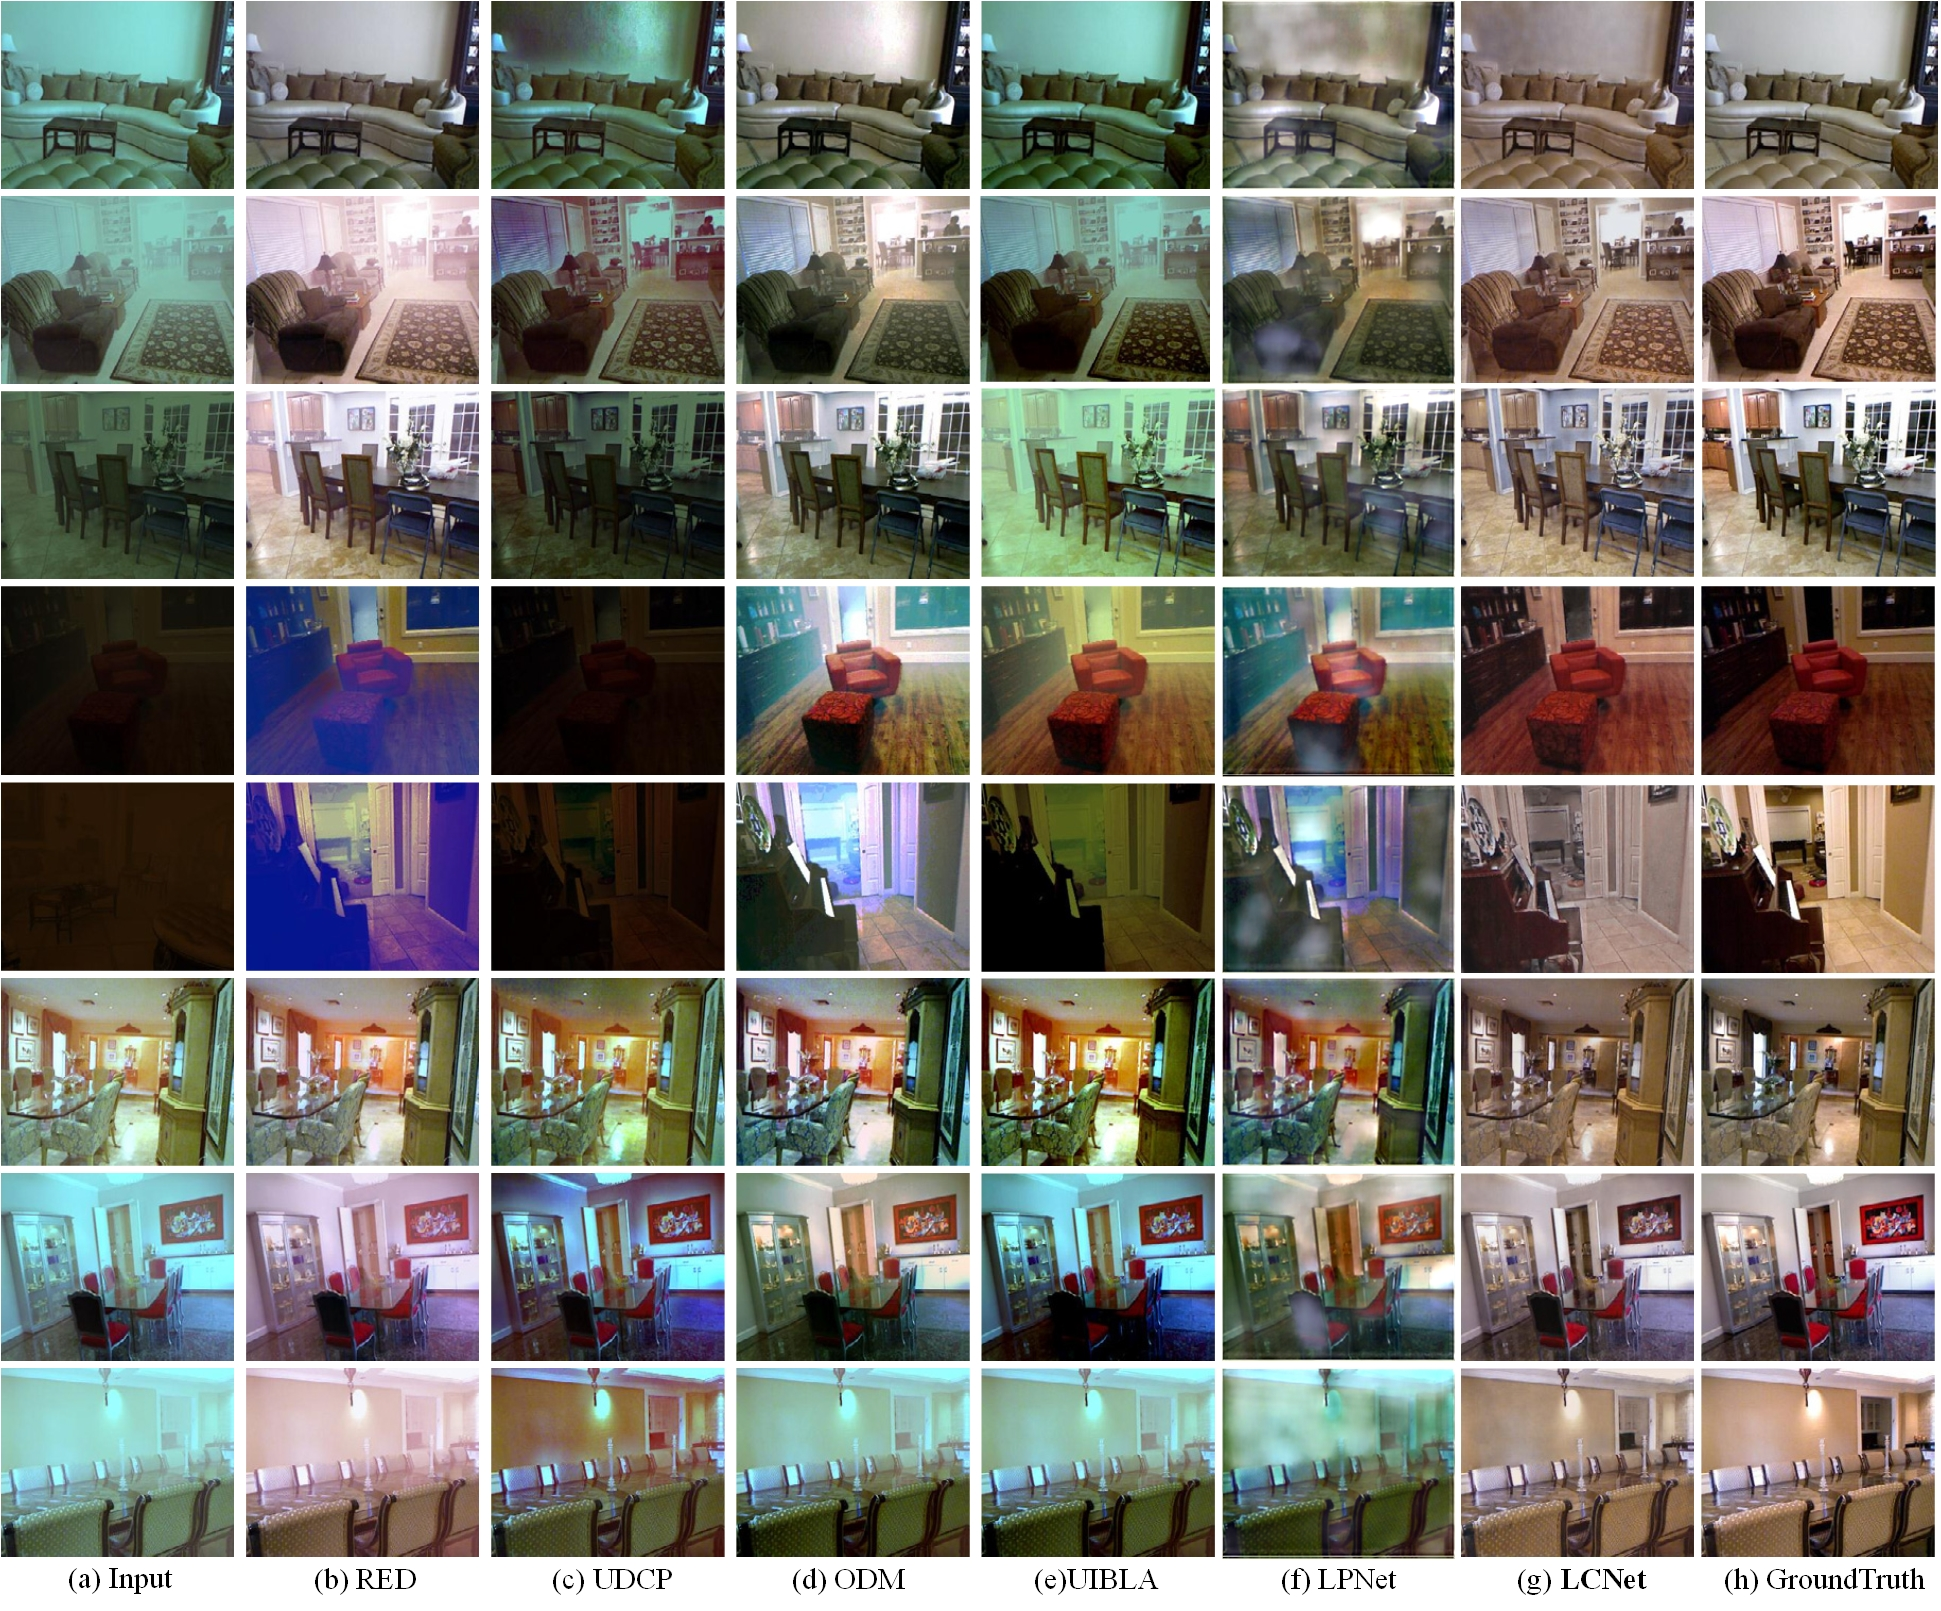
\includegraphics[width=0.9\textwidth]{Figs/Fig5.jpg}

}          
\caption{Full-reference visual comparisons of six UIE methods performed on eight synthetic images.}
\label{Fig5} 
\end{figure*} 





 \subsection{Loss Function}
To achieve both good subjective visual quality and high fidelity, we combine Mean Square Error (MSE) loss and Perceptual (PER) loss to guide the training of our network. We initialize training image pairs \(\left \{ I^{i}, I_{gt}^{i}\right \}_{i=1}^{K}\), where \(I_{gt}\) is the ground-truth, and \(K\) denotes the number of the training images.

The MSE metric is a widely used loss function in many low-level tasks (\textit{e.g.,} super-resolution, image deraining). It can be expressed as  
\begin{equation}
 L_{mse}=\frac{1}{K}\sum_{i=1}^{K}\left \| {\rm LCN}(I^{i}) - I_{gt}^{i} \right \|_{2}^{2}.
\end{equation}

However, training with the MSE loss only might lead to over-smoothed results. To avoid this problem, we combine it with a perceptual loss \cite{johnson2016perceptual}, which measures the feature difference between our predicted output and ground-truth. Similar to \cite{water-net,johnson2016perceptual}, we input the two images into a pre-trained VGG16 \cite{VGG16} network and calculate their feature difference:
\begin{equation}
\begin{aligned}
  L_{per} &=\frac{1}{K} \sum_{i=1}^{K}\frac{1}{C_{j} H_{j}W_{j}} \left \|V_{j} ({\rm LCN}(I^{i})) - V_{j}(I_{gt}^{i})\right \|_{2}^{2},\\
 \end{aligned}
\end{equation}
where \(C_{j}\)\(H_{j}\)\(W_{j}\) represents the dimension of the feature map at
\(j\)-th convolution layer within the VGG16 network, and \(V_{j}(X)\) represents the feature of the \(j\)-th convolutional layer. In particular, we focus on the last convolutional layer of VGG16 only. It is noted that the VGG16 model accepts multi-channel inputs and thus the perceptual loss can be utilized for color image processing. Finally, the above two functions are summed up to obtain the overall loss:
\begin{equation}
 L_{loss} = L_{mse} + \lambda *L_{per},\\
\end{equation}
where \(\lambda\) = 0.02 is set empirically, according to \cite{dehazeli2018single}. The effects of \(\lambda\) will be demonstrated in Table \ref{tab9} of Section IV-E.




\subsection{Parameter Settings}
The parameters involved in our model include the model and training parameters. In the model parameters, we set the number of pyramid levels \(N\) = 4, the number of recursive blocks \(b\) = 4 and the weight for loss function \(\lambda\) = 0.02. Ablation studies on these parameters are provided in Section IV-E. As for activation function, we use LReLUs with a small negative slope of 0.1. For training, We randomly generate one million 80 \(\times\) 80 patch pairs. We use the Adam optimizer \cite{kingma2014adam} with default settings: alpha = 0.001, beta1 = 0.9, beta2 = 0.999 and epsilon = \(10^{-8}\). The initial learning rate and epochs are set to 0.001 and 3, respectively. The whole model is trained in an end-to-end manner.








% \begin{table}[htbp]
%\caption{The average precision \(\%\) of object detetcion.}
%\centering
%\begin{tabular}{|c|c|c|} 
%\hline
%Methods&Original Image&Enhanced Image\\
%\hline
%Average Precision (\(\%\)) &87.2\(\%\) &93.8\(\%\)  \\
%\hline 
%\end{tabular}
%\label{tableo} 
%\end{table}



\begin{table*}[htbp]
\caption{Quantitative results evaluated on synthetic underwater images (PSNR \(\uparrow\) and SSIM \(\uparrow\)). }
\resizebox{\textwidth}{30mm}{
\begin{tabular}{|c|cc|cc|cc|cc|cc|cc|cc|cc|}
\hline
                             & \multicolumn{2}{c|}{1}                                      & \multicolumn{2}{c|}{3}                                      & \multicolumn{2}{c|}{5}                                       & \multicolumn{2}{c|}{7}                                      & \multicolumn{2}{c|}{9}                                      & \multicolumn{2}{c|}{\uppercase\expandafter{\romannumeral1}}                                      & \multicolumn{2}{c|}{\uppercase\expandafter{\romannumeral2}}                                       & \multicolumn{2}{c|}{\uppercase\expandafter{\romannumeral3}}                                      \\ \cline{2-17} 
\multirow{-2}{*}{Water Type} & PSNR                         & SSIM                         & PSNR                         & SSIM                         & PSNR                         & SSIM                         & PSNR                         & SSIM                         & PSNR                         & SSIM                         & PSNR                         & SSIM                         & PSNR                         & SSIM                         & PSNR                         & SSIM                         \\ \hline
RAW                          & \multicolumn{1}{l}{15.53}    & \multicolumn{1}{l|}{0.765}   & \multicolumn{1}{l}{14.69}    & \multicolumn{1}{l|}{0.629}   & \multicolumn{1}{l}{12.14}    & \multicolumn{1}{l|}{0.502}   & \multicolumn{1}{l}{10.17}    & \multicolumn{1}{l|}{0.519}   & \multicolumn{1}{l}{9.50}     & \multicolumn{1}{l|}{0.302}   & \multicolumn{1}{l}{17.36}    & \multicolumn{1}{l|}{0.886}   & \multicolumn{1}{l}{20.59}    & \multicolumn{1}{l|}{0.868}   & \multicolumn{1}{l}{16.55}    & \multicolumn{1}{l|}{0.788}   \\
Fusion-Based \cite{fusion-based}                & 15.79                        & 0.706                        & 15.01                        & 0.578                        & 13.19                        & 0.421                        & 11.02                        & 0.279                        & 10.76                        & 0.179                        & 18.38                        & 0.862                        & 20.88                        & 0.871                        & 17.12                        & 0.752                        \\
RED \cite{RED}                       & 15.90                        & 0.741                        & 12.79                        & 0.663                        & 11.12                        & 0.593                        & 9.99                         & 0.508                        & 11.62                        & 0.319                        & 19.54                        & 0.881                        & 20.79                        & 0.883                        & 16.69                        & 0.791                        \\
UDCP \cite{UDCP}                       & 15.76                        & 0.763                        & 14.47                        & 0.661                        & 10.86                        & 0.426                        & 9.47                         & 0.262                        & 9.32                         & 0.162                        & 18.82                        & 0.826                        & 17.20                        & 0.838                        & 14.92                        & 0.758                        \\
ODM \cite{Histogram-prior}                        & 16.09                        & 0.724                        & 14.28                        & 0.676                        & 14.12                        & 0.644                        & 12.27                        & 0.563                        & 9.30                         & 0.417                        & 18.09                        & 0.817                        & 17.61                        & 0.825                        & 16.71                        & 0.754                        \\
GDCP \cite{GDCP}                         & 15.89                        & 0.779                        & 17.45                        & 0.706                        & 12.89                        & 0.687                        & 12.47                        & 0.613                        & 13.08                        & 0.462                        & 21.42                        & 0.826                        & 23.20                        & 0.832                        & 18.92                        & 0.828                        \\
Retinex-Based \cite{fu2014retinex}              & 16.02                        & 0.735                        & 15.81                        & 0.688                        & 13.53                        & 0.625                        & 12.02                        & 0.679                        & 12.16                        & 0.455                        & 20.58                        & 0.862                        & 22.19                        & 0.892                        & 17.75                        & 0.791                        \\
UIBLA \cite{blurriness-based}                       & 15.88                        & 0.695                        & 13.44                        & 0.576                        & 12.61                        & 0.474                        & 10.75                        & 0.305                        & 10.09                        & 0.220                        & 17.49                        & 0.744                        & 18.06                        & 0.801                        & 17.10                        & 0.765                        \\
LPNet \cite{fu2019lightweight}                      & 18.38                        & 0.755                        & 13.71                        & 0.663                        & 13.01                        & 0.558                        & 10.37                        & 0.466                        & 10.33                        & 0.373                        & 17.87                        & 0.812                        & 18.35                        & 0.857                        & 17.49                        & 0.807                        \\
Ancuti \textit{et al.}(2016) \cite{ancuti2016multi}                        & 16.22                        & 0.651                        & 14.12                        & 0.593                        & 12.98                        & 0.532                        & 11.31                        & 0.499                        & 11.45                        & 0.391                        & 17.12                        & 0.801                        & 18.12                        & 0.831                        & 17.11                        & 0.801                        \\
Ancuti \textit{et al.}(2017) \cite{ancuti2017color}                      & 16.41                        & 0.677                        & 14.33                        & 0.599                        & 13.31                        & 0.542                        & 11.66
& 0.512                        & 11.55                        & 0.401                        & 17.35                        & 0.803                        & 18.22
& 0.840                        & 17.21                        & 0.808 \\
Berman \textit{et al.}(2020) \cite{berman2020underwater}                       & 17.01                        & 0.702                        & 14.82                        & 0.613                        & 13.62                        & 0.581                        & 12.01                        & 0.532                       & 11.86                        & 0.489                        & 17.66                        & 0.811                        & 18.63                        & 0.861                        & 17.65                        & 0.812                        \\
Water-CycleGAN \cite{water-gan}               & 17.19                        & 0.789                        & 19.18                        & 0.776                        & 17.32                        & 0.758                        & 14.32                        & 0.683                        & 12.15                        & 0.517                        & 22.89                        & 0.817                        & 24.61                        & 0.837                        & 19.66                        & {\color[HTML]{3166FF} 0.889} \\
Dense-GAN \cite{dense-gan}                   & 19.88                        & 0.815                        & 14.15                        & 0.793                        & 17.51                        & {\color[HTML]{3166FF} 0.819} & 14.13                        & 0.712                        & 13.09                        & {\color[HTML]{3166FF} 0.620} & 23.99                        & 0.882                        & 23.06                        & 0.821                        & 20.15                        & 0.862                        \\
Water-Net \cite{water-net}                    & 19.15                        & 0.832                        & 14.39                        & {\color[HTML]{3166FF} 0.805} & 17.11                        & {\color[HTML]{FE0000} 0.822} & 14.16                        & {\color[HTML]{3166FF} 0.785} & 13.21                        & 0.613                        & 24.17                        & {\color[HTML]{3166FF} 0.898} & 24.35                        & 0.862                        & 20.29                        & 0.833                        \\
UWCNN \cite{uwcnn}                        & {\color[HTML]{3166FF} 21.79} & {\color[HTML]{3166FF} 0.850} & {\color[HTML]{3166FF} 20.25} & 0.795                        & {\color[HTML]{3166FF} 17.52} & 0.726                        & {\color[HTML]{3166FF} 14.22} & 0.607                        & {\color[HTML]{3166FF} 13.23} & 0.492                        & {\color[HTML]{3166FF} 25.93} & {\color[HTML]{FE0000} 0.937} & {\color[HTML]{3166FF} 24.82} & {\color[HTML]{FE0000} 0.923} & {\color[HTML]{3166FF} 22.63} & 0.879                        \\
\textbf{LCNet}                & {\color[HTML]{FE0000} 22.14} & {\color[HTML]{FE0000} 0.876} & {\color[HTML]{FE0000} 23.38} & {\color[HTML]{FE0000} 0.832} & {\color[HTML]{FE0000} 22.35} & 0.816                        & {\color[HTML]{FE0000} 21.55} & {\color[HTML]{FE0000} 0.797} & {\color[HTML]{FE0000} 21.46} & {\color[HTML]{FE0000} 0.651} & {\color[HTML]{FE0000} 26.34} & 0.895                        & {\color[HTML]{FE0000} 25.28} & {\color[HTML]{3166FF} 0.907} & {\color[HTML]{FE0000} 23.18} & {\color[HTML]{FE0000} 0.916} \\ \hline
\end{tabular}}
\label{tab1} 
\end{table*}


\begin{table*}[htbp]
\caption{Quantitative results evaluated on synthetic underwater images (MSE \(\downarrow\) and LPIPS \(\downarrow\)). }
\resizebox{\textwidth}{30mm}{
\begin{tabular}{|c|cc|cc|cc|cc|cc|cc|cc|cc|}
\hline
                             & \multicolumn{2}{c|}{1}                                      & \multicolumn{2}{c|}{3}                                      & \multicolumn{2}{c}{5}                                        & \multicolumn{2}{c|}{7}                                       & \multicolumn{2}{c|}{9}                                       & \multicolumn{2}{c|}{\uppercase\expandafter{\romannumeral1}}                                      & \multicolumn{2}{c}{\uppercase\expandafter{\romannumeral2}}                                       & \multicolumn{2}{c|}{\uppercase\expandafter{\romannumeral3}}                                      \\ \cline{2-17} 
\multirow{-2}{*}{Water Type} & MSE                          & LPIPS                        & MSE                          & LPIPS                        & MSE                           & LPIPS                        & MSE                           & LPIPS                        & MSE                           & LPIPS                        & MSE                          & LPIPS                        & MSE                          & LPIPS                        & MSE                          & LPIPS                        \\ \hline
RAW                          & \multicolumn{1}{l}{2367.3}   & \multicolumn{1}{l|}{0.246}   & \multicolumn{1}{l}{2676.5}   & \multicolumn{1}{l|}{0.453}   & \multicolumn{1}{l}{4851.2}    & \multicolumn{1}{l|}{0.393}   & \multicolumn{1}{l}{7381.1}    & \multicolumn{1}{l|}{0.502}   & \multicolumn{1}{l}{9060.6}    & \multicolumn{1}{l|}{0.713}   & \multicolumn{1}{l}{1449.0}   & \multicolumn{1}{l|}{0.242}   & \multicolumn{1}{l}{941.9}    & \multicolumn{1}{l|}{0.253}   & \multicolumn{1}{l}{1851.0}   & \multicolumn{1}{l|}{0.421}   \\
Fusion-Based \cite{fusion-based}                & 2258.3                       & 0.227                        & 2836.5                       & 0.442                        & 3218.5                        & 0.312                        & 5835.8                        & 0.425                        & 7895.4                        & 0.632                        & 1239.2                       & 0.208                        & 747.2                        & 0.192                        & 1293.4                       & 0.386                        \\
RED \cite{RED}                         & 3489.7                       & 0.126                        & 4953.2                       & 0.281                        & 8385.8                        & 0.233                        & 9809.8                        & 0.423                        & 5952.3                        & 0.427                        & 936.9                        & 0.241                        & 851.3                        & 0.177                        & 2240.0                       & 0.241                        \\
UDCP \cite{UDCP}                        & 2062.3                       & 0.304                        & 3380.6                       & 0.277                        & 6708.9                        & 0.319                        & 8591.6                        & 0.414                        & 9500.1                        & 0.458                        & 1020.7                       & 0.234                        & 1466.9                       & 0.229                        & 2337.6                       & 0.245                        \\
ODM \cite{Histogram-prior}                         & 2508.6                       & 0.117                        & 3130.1                       & 0.268                        & 3488.9                        & 0.142                        & 5337.1                        & 0.410                        & 10634.0                       & 0.230                        & 1272.0                       & 0.239                        & 1401.9                       & 0.171                        & 1701.1                       & 0.326                        \\
GDCP \cite{GDCP}                         & 1877.4                       & 0.152                        & 2542.2                       & 0.252                        & 2799.5                        & 0.289                        & 3578.9                        & 0.394                        & 3528.1                        & 0.458                        & 738.9                        & 0.202                        & 811.2                        & 0.194                        & 1788.4                       & 0.227                        \\
Retinex-Based \cite{fu2014retinex}               & 2149.2                       & 0.193                        & 1677.9                       & 0.423                        & 3009.2                        & 0.232                        & 4766.2                        & 0.395                        & 4312.7                        & 0.659                        & 1128.2                       & 0.218                        & 658.3                        & 0.181                        & 1031.2                       & 0.312                        \\
UIBLA \cite{blurriness-based}                       & 2812.6                       & 0.207                        & 3490.1                       & 0.368                        & 4563.7                        & 0.330                        & 6737.9                        & 0.299                        & 8433.1                        & 0.265                        & 1492.2                       & 0.237                        & 1141.4                       & 0.225                        & 1697.8                       & 0.319                        \\
LPNet \cite{fu2019lightweight}                       & 2502.2                       & 0.254                        & 3217.8                       & 0.373                        & 4105.2                        & 0.219                        & 5832.7                        & 0.408                        & 8722.7                        & 0.252                        & 1099.6                       & 0.278                        & 1022.5                       & 0.264                        & 1487.2                       & 0.397                        \\
Ancuti \textit{et al.}(2016) \cite{ancuti2016multi}  & 1365.8                       & 0.354                        & 2917.2                       & 0.311                        & 4615.2                        & 0.232                       & 3812.5                        & 0.412                        & 7739.7                        & 0.253                        & 1126.3                       & 0.277                        & 1121.5                       & 0.292                        & 1827.1                       & 0.401                        \\
Ancuti \textit{et al.}(2017) \cite{ancuti2017color}   & 1347.2                       & 0.313                        & 2527.2                       & 0.302                        & 4533.2                        & 0.212                       & 3202.3                       & 0.396                        & 7255.9                        & 0.241                        & 1109.2                       & 0.262                        & 1002.4                       & 0.263                        & 1617.1                       & 0.381                        \\
Berman \textit{et al.}(2020) \cite{berman2020underwater} & 1042.3                       & 0.301                        & 2217.2                       & 0.282                        & 3833.6                        & 0.201                       & 2811.7                       & 0.312                        & 6651.4                        & 0.223                        & 899.2                       & 0.249                        & 898.1                        & 0.254                 
&1482.1                       & 0.361                        \\
Water-CycleGAN \cite{water-gan}              & 655.3                        & 0.168                        & 698.2                        & 0.168                        & 867.5                         & 0.141                        & 1423.7                        & 0.380                        & 1247.9                        & 0.370                        & 876.2                        & 0.142                        & 1232.9                       & 0.162                        & {\color[HTML]{FE0000} 338.9} & {\color[HTML]{343434} 0.233} \\
Dense-GAN \cite{dense-gan}                    & 609.2                        & 0.113                        & 536.7                        & 0.149                        & {\color[HTML]{FE0000} 409.5}  & {\color[HTML]{343434} 0.165} & 1028.3                        & 0.199                        & 865.3                         & {\color[HTML]{343434} 0.365} & 213.6                        & {\color[HTML]{343434} 0.138} & {\color[HTML]{FE0000} 203.8} & {\color[HTML]{3166FF} 0.125} & 411.2                        & 0.222                        \\
Water-Net \cite{water-net}                   & 586.2                        & {\color[HTML]{3166FF} 0.112} & {\color[HTML]{3166FF} 402.3} & {\color[HTML]{343434} 0.176} & 616.5                         & {\color[HTML]{343434} 0.171} & {\color[HTML]{3166FF} 785.6}  & {\color[HTML]{343434} 0.130} & {\color[HTML]{3166FF} 799.3}  & 0.434                        & 455.9                        & {\color[HTML]{3166FF} 0.112} & 223.4                        & 0.155                        & 452.9                        & {\color[HTML]{3166FF} 0.134} \\
UWCNN \cite{uwcnn}                       & {\color[HTML]{3166FF} 587.7} & {\color[HTML]{343434} 0.200} & {\color[HTML]{343434} 747.5} & {\color[HTML]{3166FF} 0.192} & {\color[HTML]{343434} 1295.1} & {\color[HTML]{FE0000} 0.114} & {\color[HTML]{343434} 2974.1} & {\color[HTML]{FE0000} 0.123} & {\color[HTML]{343434} 4121.5} & {\color[HTML]{3166FF} 0.218} & {\color[HTML]{3166FF} 209.7} & {\color[HTML]{343434} 0.123} & {\color[HTML]{343434} 251.6} & {\color[HTML]{343434} 0.176} & {\color[HTML]{343434} 456.4} & {\color[HTML]{FE0000} 0.114} \\
\textbf{LCNet}                & {\color[HTML]{FE0000} 467.7} & {\color[HTML]{FE0000} 0.107} & {\color[HTML]{FE0000} 398.2} & {\color[HTML]{FE0000} 0.146} & {\color[HTML]{3166FF} 427.9}  & {\color[HTML]{3166FF} 0.135} & {\color[HTML]{FE0000} 613.7}  & {\color[HTML]{3166FF} 0.128} & {\color[HTML]{FE0000} 598.3}  & {\color[HTML]{FE0000} 0.215} & {\color[HTML]{FE0000} 137.5} & {\color[HTML]{FE0000} 0.097} & {\color[HTML]{3166FF} 205.7} & {\color[HTML]{FE0000} 0.102} & {\color[HTML]{3166FF} 376.9} & 0.397 \\ \hline
\end{tabular}
}
\label{tab2}
\end{table*}


\begin{figure*}[h] 
\centering 
{   
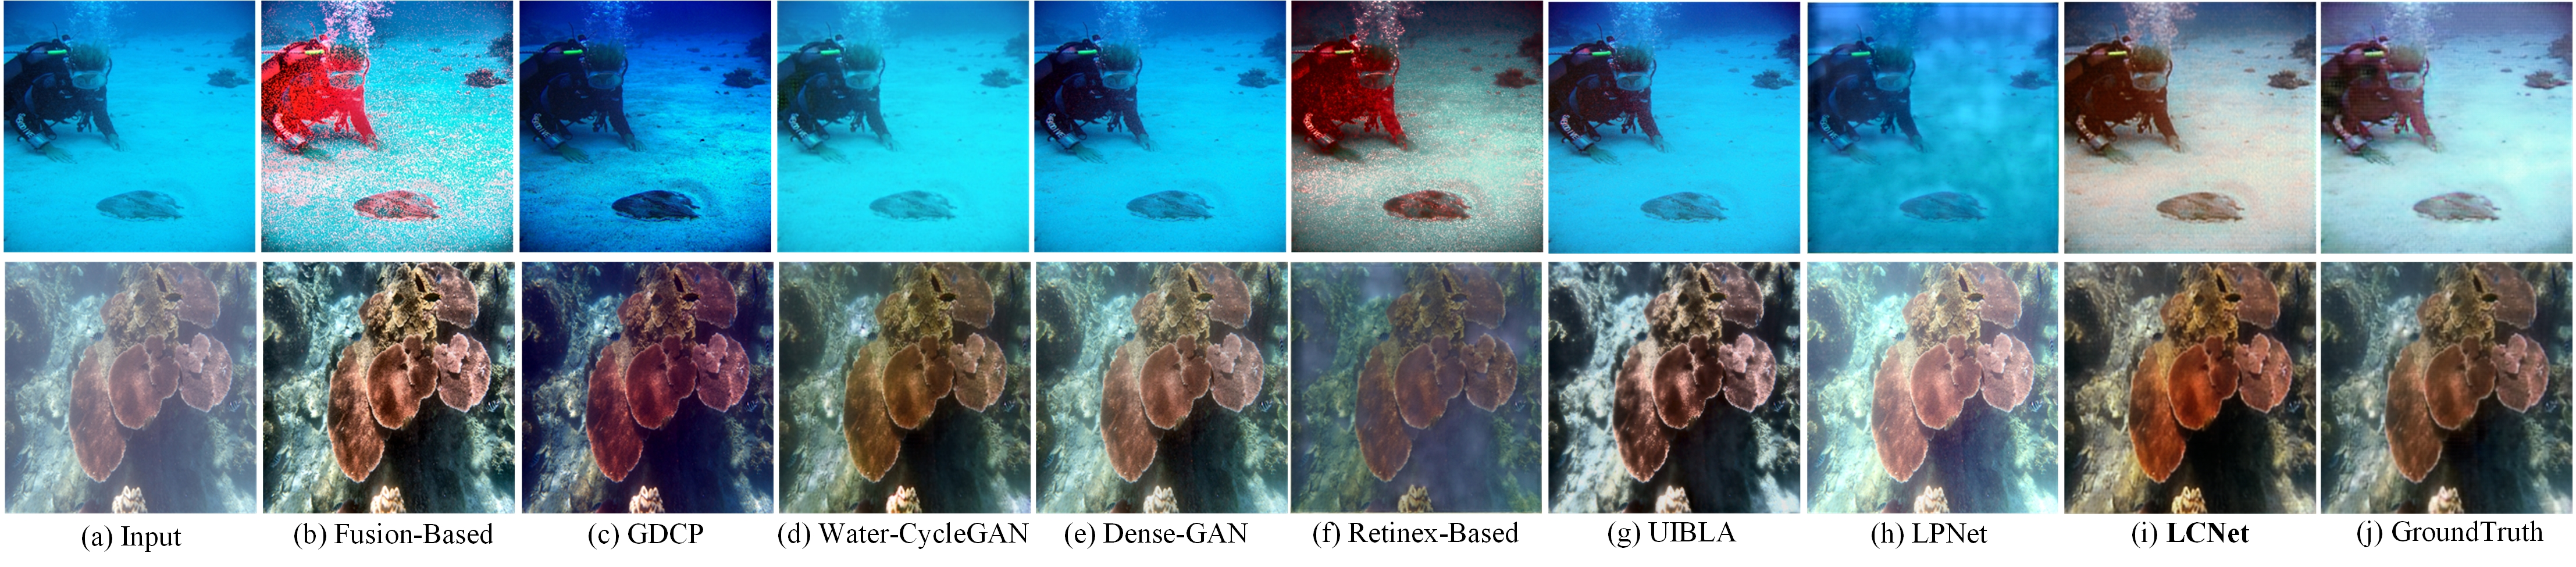
\includegraphics[width=1\textwidth]{Figs/Fig6.jpg}

}          
\caption{Visual qualitative comparisons on real-world images.}
\label{Fig6} 
\end{figure*} 

\begin{figure*}[h] 
\centering 
{   
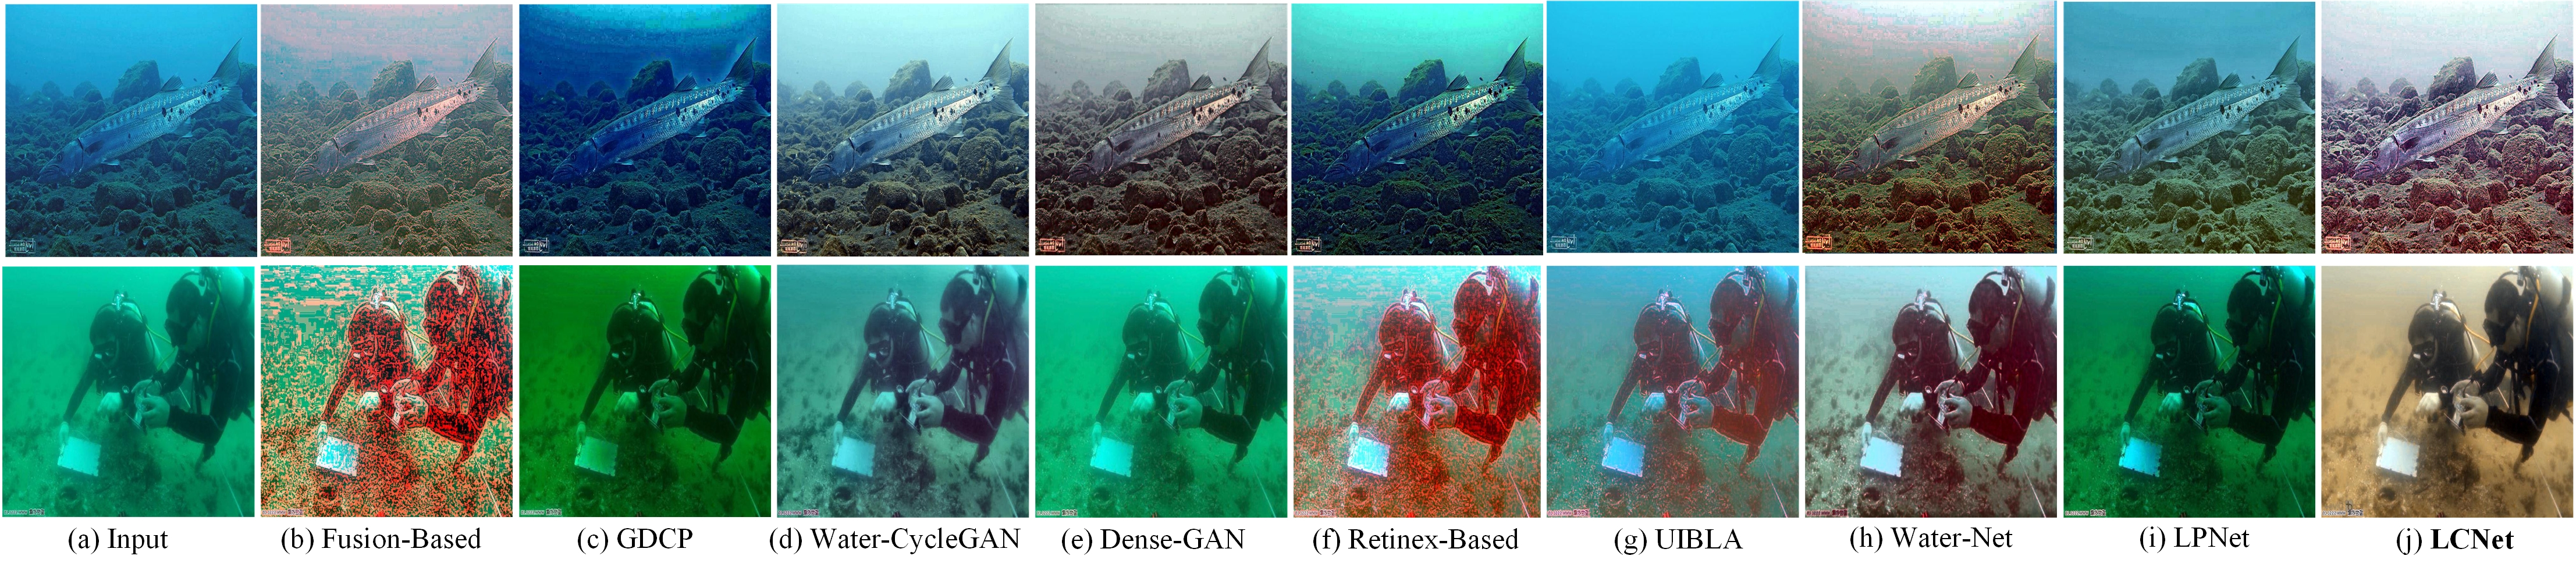
\includegraphics[width=0.95\textwidth]{Figs/Fig7.jpg}

}          
\caption{Visual qualitative comparisons on challenging set.}
\label{Fig7} 
\end{figure*} 


\section{Experimental Results}
In this section, we evaluate the proposed method and compare it with several state-of-the-art UIE methods on both synthetic and real-world underwater images. 

\subsection{Compared Algorithms}
We choose 15 popular algorithms for comparison, including Fusion-Based \cite{fusion-based}, RED \cite{RED}, UDCP \cite{UDCP}, ODM \cite{Histogram-prior}, UIBLA \cite{blurriness-based}, LPNet \cite{fu2019lightweight}, UWCNN \cite{uwcnn}, Retinex-Based \cite{fu2014retinex}, GDCP \cite{GDCP}, Ancuti \textit{et al.} (2016) \cite{ancuti2016multi}, Ancuti \textit{et al.} (2017)\cite{ancuti2017color}, Berman \textit{et al.} (2020)\cite{berman2020underwater}, Water-CycleGAN \cite{water-gan}, Dense-GAN \cite{dense-gan} and Water-Net\cite{water-net}. Among them, \cite{ancuti2016multi,ancuti2017color,fusion-based} are non-physics model-based methods, \cite{UDCP,GDCP,blurriness-based,ancuti2016multi,Histogram-prior,berman2020underwater,fu2014retinex} are physics model-based methods and \cite{fu2019lightweight,uwcnn,water-gan,dense-gan,water-net} are deep learning-based methods. All experiments (Training/Testing) are performed on a server equipped with two NVIDIA GeForce GTX 2080Ti with 16GB GPU memory. The size of images are set to 512 \(\times\) 512.

\begin{table}[h]
\caption{Quantitative results evaluated on real-world dataset UIEB. }
\centering
\begin{tabular}{|c|c|c|c|c|} 
\hline
Methods&PSNR\(\uparrow\)&SSIM\(\uparrow\)&MSE\(\downarrow\)&LPIPS\(\downarrow\)\\
\hline
Fusion-Based \cite{fusion-based} &17.61 &0.772 &1128.0&0.344 \\
\hline 
RED \cite{RED} &17.89 &0.793 &933.2&0.298 \\
\hline 
UDCP \cite{UDCP} &18.79 &0.811 &897.2&0.295 \\
\hline 
ODM \cite{Histogram-prior} &15.82&0.539&1701.9&0.382\\
\hline
UIBLA \cite{blurriness-based} &15.32&0.603&1911.1&0.311\\
\hline
LPNet \cite{fu2019lightweight} &15.65 &0.714 &1671.3&0.396 \\
\hline 
UWCNN \cite{uwcnn} &19.08 &\textcolor{blue}{0.812}&\textcolor{blue}{766.1}&0.344 \\
\hline
Retinex-Based \cite{fu2014retinex} &17.02&0.607&1292.4&0.537\\
\hline 
GDCP \cite{GDCP} &12.09 &0.512 &1010.0&0.770\\
\hline
Ancuti \textit{et al.}(2016) \cite{ancuti2016multi} &15.12 &0.602&1324.2&0.612 \\
\hline
Ancuti \textit{et al.}(2017) \cite{ancuti2017color} &15.58 &0.724&1466.2&0.649 \\
\hline
Berman \textit{et al.}(2020) \cite{berman2020underwater} &16.11 &0.711&1320.9&0.596 \\
\hline
Water-CycleGAN \cite{water-gan} &15.75&0.521&1729.8&0.348\\
\hline
Dense-GAN \cite{dense-gan}&17.28&0.443&1215.2&0.318\\
\hline
Water-Net \cite{water-net} &\textcolor{blue}{19.11}&0.797&797.6&\textcolor{red}{0.222}\\
\hline
\textbf{LCNet}&\textcolor{red}{23.22}&\textcolor{red}{0.923}&\textcolor{red}{573.6}&\textcolor{blue}{0.287}\\
\hline 
\end{tabular}

\label{tab3} 
\end{table}




\subsection{Datasets}
\textbf{Synthetic Underwater Image Dataset}. We train the proposed network on synthetic images from \cite{uwcnn} which were generated using the attenuation coefficients described in \cite{berman2017diving}. This dataset contains 10 different water types of oceanic and coastal classes (\textit{i.e.}, I, IA, IB, II, and III for open ocean waters, and 1, 3, 5, 7, and 9 for coastal waters). Each type consists of 1449 images, in which we randomly select 1000 images as training set and the remaining 449 images as testing set.

\textbf{Real-World Underwater Image Dataset}. We also use the UIEB
real-world dataset built in \cite{water-net} to evaluate different methods. These images are collected from Google and YouTube, and their corresponding reference images are generated by 15 image enhancement methods. The final versions of images are provided according to
well-designed pairwise comparisons. This dataset consists of 890 underwater images with their corresponding high-quality reference images, in which a random set of 800 pairs of the images are used for training and the rest 90 images are used for testing. Besides, it also contains 60 challenging underwater images for non-reference quality evaluation. Recently, a new underwater dataset, named Stereo Quantitative Underwater Image Dataset (SQUID), was proposed in \cite{berman2020underwater}. The dataset contains 57 stereo pairs from four different sites in Israel and takes into account multiple spectral profiles of different water types. In addition, this dataset is only used for non-reference evaluation.


\begin{table}[h]
 \caption{Non-reference image quality evaluations on challenge set of UIEB \cite{water-net}. }
\centering

\begin{tabular}{|c|c|c|c|c|} 
\hline 
Methods&UCIQE\(\uparrow\)&UIQM\(\uparrow\)&CCF\(\uparrow\)&ILNIQE\(\uparrow\)\\
\hline
Fusion-Based \cite{fusion-based}&0.6414&\textcolor{blue}{1.5310}&15.0811&0.4695 \\
\hline
RED \cite{RED} &0.6355&1.489&14.1922&0.5733 \\
\hline 
UDCP \cite{UDCP} &0.6216&1.435&14.2943&0.5812 \\
\hline 
ODM \cite{Histogram-prior} &\textcolor{red}{0.6778}&\textcolor{red}{1.5440}&6.0821&0.5768\\
\hline
UIBLA \cite{blurriness-based} &0.6001&1.3757&\textcolor{blue}{15.7701}&0.4619\\
\hline
LPNet \cite{fu2019lightweight} &0.6221&1.2782&9.1002&0.4724\\
\hline
UWCNN \cite{uwcnn} &0.6328&1.5082&12.3402&0.6579\\
\hline
Retinex-Based \cite{fu2014retinex} &0.6062&1.4338&13.4510&0.4911\\
\hline
GDCP \cite{GDCP}&0.5993 &1.4301&12.0734&0.4979 \\
\hline
Ancuti \textit{et al.}(2016) \cite{ancuti2016multi} &0.6001 &1.3908&13.2439&0.5100 \\
\hline
Ancuti \textit{et al.}(2017) \cite{ancuti2017color} &0.5872 &1.4871&12.9912&0.5495 \\
\hline
Berman \textit{et al.}(2020) \cite{berman2020underwater} &0.6231 &1.4118&13.1212&0.5766 \\
\hline
Water-CycleGAN \cite{water-gan} &0.5656&1.4376&12.1455&0.6386\\
\hline
Dense-GAN \cite{dense-gan} & 0.6419&1.5467&13.4732&0.6051\\
\hline
Water-Net \cite{water-net} &0.6110&1.4640&10.3101&\textcolor{blue}{0.6566}
\\
\hline
\textbf{LCNet}&\textcolor{blue}{0.6449} &1.4096&\textcolor{red}{16.2102}&\textcolor{red}{0.6919}
\\
\hline 
\end{tabular}
\label{tab4} 
\end{table}

\begin{table}[h]
 \caption{Non-reference image quality evaluations on SQUID \cite{berman2020underwater}.}
\centering

\begin{tabular}{|c|c|c|c|c|} 
\hline 
Methods&UCIQE\(\uparrow\)&UIQM\(\uparrow\)&CCF\(\uparrow\)&ILNIQE\(\uparrow\)\\
\hline
Fusion-Based \cite{fusion-based}&0.6237&\textcolor{red}{1.6110}&\textcolor{blue}{15.2312}&0.5012 \\
\hline
RED \cite{RED}&0.6122&1.308&13.2317&0.4723 \\
\hline 
UDCP \cite{UDCP} &0.5916&1.277&10.3243&0.3812 \\
\hline 
ODM \cite{Histogram-prior}&0.5782&1.3480&7.2831&0.5668\\
\hline
UIBLA \cite{blurriness-based}&0.4988&1.4297&15.6901&0.3939\\
\hline
LPNet \cite{fu2019lightweight} &0.6119&1.2213&9.1002&0.4724\\
\hline
UWCNN \cite{uwcnn}&\textcolor{blue}{0.6738}&1.5342&11.5422&0.6012\\
\hline
Retinex-Based \cite{fu2014retinex} &0.6179&1.4125&12.1599&0.4232\\
\hline
GDCP \cite{GDCP}&0.5803 &1.2931&13.1924&0.4979 \\
\hline
Ancuti \textit{et al.}(2016) \cite{ancuti2016multi} &0.6003 &1.3915&13.2509&0.5103 \\
\hline
Ancuti \textit{et al.}(2017) \cite{ancuti2017color} &0.5885 &1.4871&12.9912&0.5512 \\
\hline
Berman \textit{et al.}(2020) \cite{berman2020underwater} &0.6252 &1.4115&13.1223&0.5779 \\
\hline
%Ancuti et al.(2018) &0.6377 &1.5133&14.2273&0.6072 \\
%\hline
%Berman et al.(2020) &0.6651 &1.5377&14.6298&0.6471 \\
%\hline
Water-CycleGAN \cite{water-gan}&0.5752&1.4188&12.1915&0.6192\\
\hline
Dense-GAN \cite{dense-gan} & 0.6529&\textcolor{blue}{1.5437}&13.4285&0.6122\\
\hline
Water-Net \cite{water-net} &0.6019&1.5123&11.4123&\textcolor{blue}{0.6896}
\\
\hline
\textbf{LCNet}&\textcolor{red}{0.6949} &1.4286&\textcolor{red}{15.7102}&\textcolor{red}{0.6989}
\\
\hline 
\end{tabular}
\label{tab5} 
\end{table}







\begin{table*}[h]
\caption{Average runtime of some selected methods. Red and blue indicate the best and second-best results.}
\centering
\setlength{\tabcolsep}{1mm}{
\begin{tabular}{|c|c|c|c|c|c|c|c|c|c|} %l(left)居左显示 r(right)居右显示 c居中显示
\hline 
Methods&Fusion-Based  &Retinex-Based  & RED  &UDCP  &ODM &Water-CycleGAN  &Water-Net  &UWCNN  &\textbf{LCNet} \\
& \cite{fusion-based} & \cite{fu2014retinex} &  \cite{RED} & \cite{UDCP} & \cite{Histogram-prior}& \cite{water-gan} & \cite{water-net} & \cite{uwcnn} & \\
\hline  
Time(s) 500\(\times\)500  &0.604&0.697&2.752&2.268&4.628&0.225&\textcolor{blue}{0.213}&0.241&\textcolor{red}{0.121}\\
Time(s) 640\(\times\)480 &0.679&0.882&3.250&3.319&5.829&0.263&\textcolor{blue}{0.228}&0.271&\textcolor{red}{0.128}\\
Time(s) 1280\(\times\) 720&1.843&2.109&9.745&9.902&16.923&0.325&\textcolor{blue}{0.282}&0.402&\textcolor{red}{0.157}\\
\hline 
Parameters&-&-&-&-&-&57,169,668&1,090,668&\textcolor{blue}{90,646}&\textcolor{red}{23,325}\\
\hline
FLOPs(M)&-&-&-&-&-&3,887,403&\textcolor{blue}{1,937,278}&3,931,010&\textcolor{red}{139,055}\\
\hline
\end{tabular}}
\label{tab6} 
\end{table*}










\begin{figure}[htbp] 
\centering 
{   
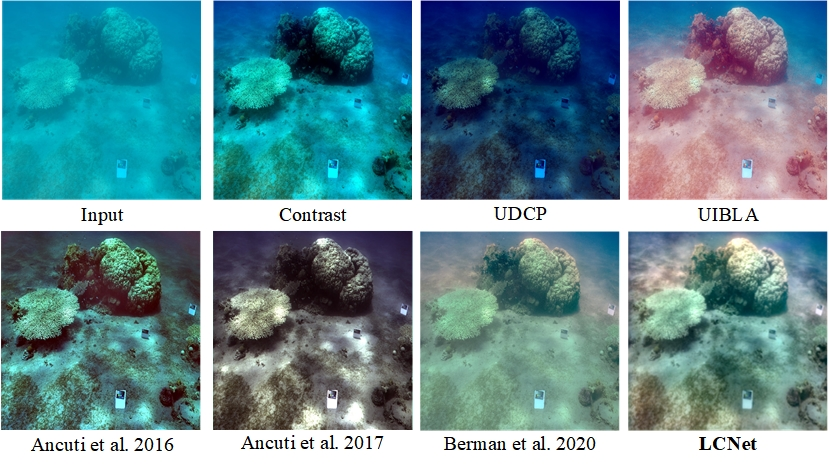
\includegraphics[width=0.45\textwidth]{Figs/Fig8.jpg}

}          
\caption{Visual qualitative results on SQUID.}
\label{Fig8} 
\end{figure} 



\begin{figure*}[ht]
\centering  %图片全局居中
\subfigure[]
{
\label{Fig.c.1}
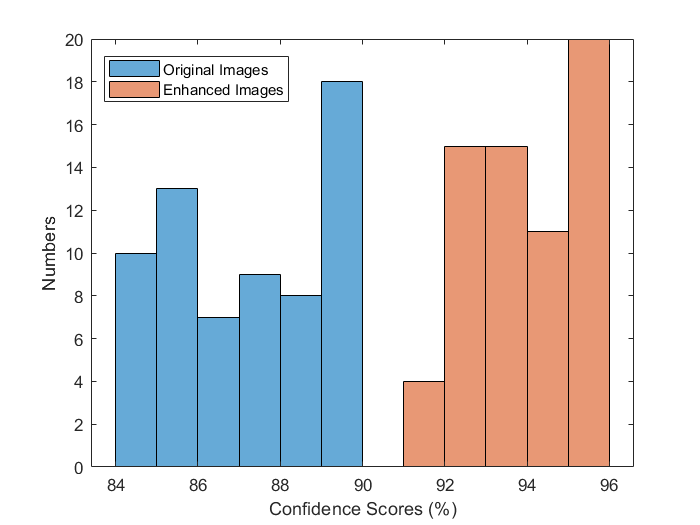
\includegraphics[width=6cm,height=5.5cm]{Figs/Fig9-1.png}
}\hspace{12mm}
\subfigure[]{
\label{Fig.c.2}
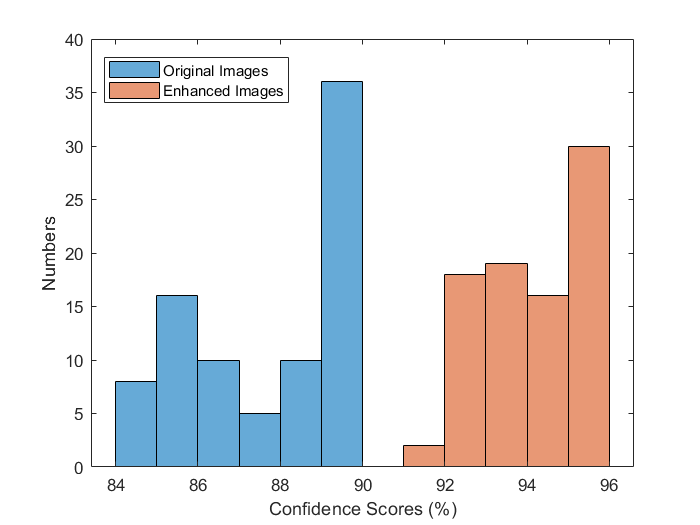
\includegraphics[width=6cm,height=5.5cm]{Figs/Fig9-2.png}}
\caption{The distributions of confidence scores of original and enhanced images. (a) Humans (87.4 $\pm$ 4.5 \(\%\) vs 93.8 $\pm$ 1.8 \(\%\)). (b) Fishes (86.7 $\pm$ 4.2 \(\%\) vs 93.5 $\pm$ 2.1 \(\%\)).}
\label{Fig9}
\end{figure*}



\begin{figure*}[h]
\centering
{
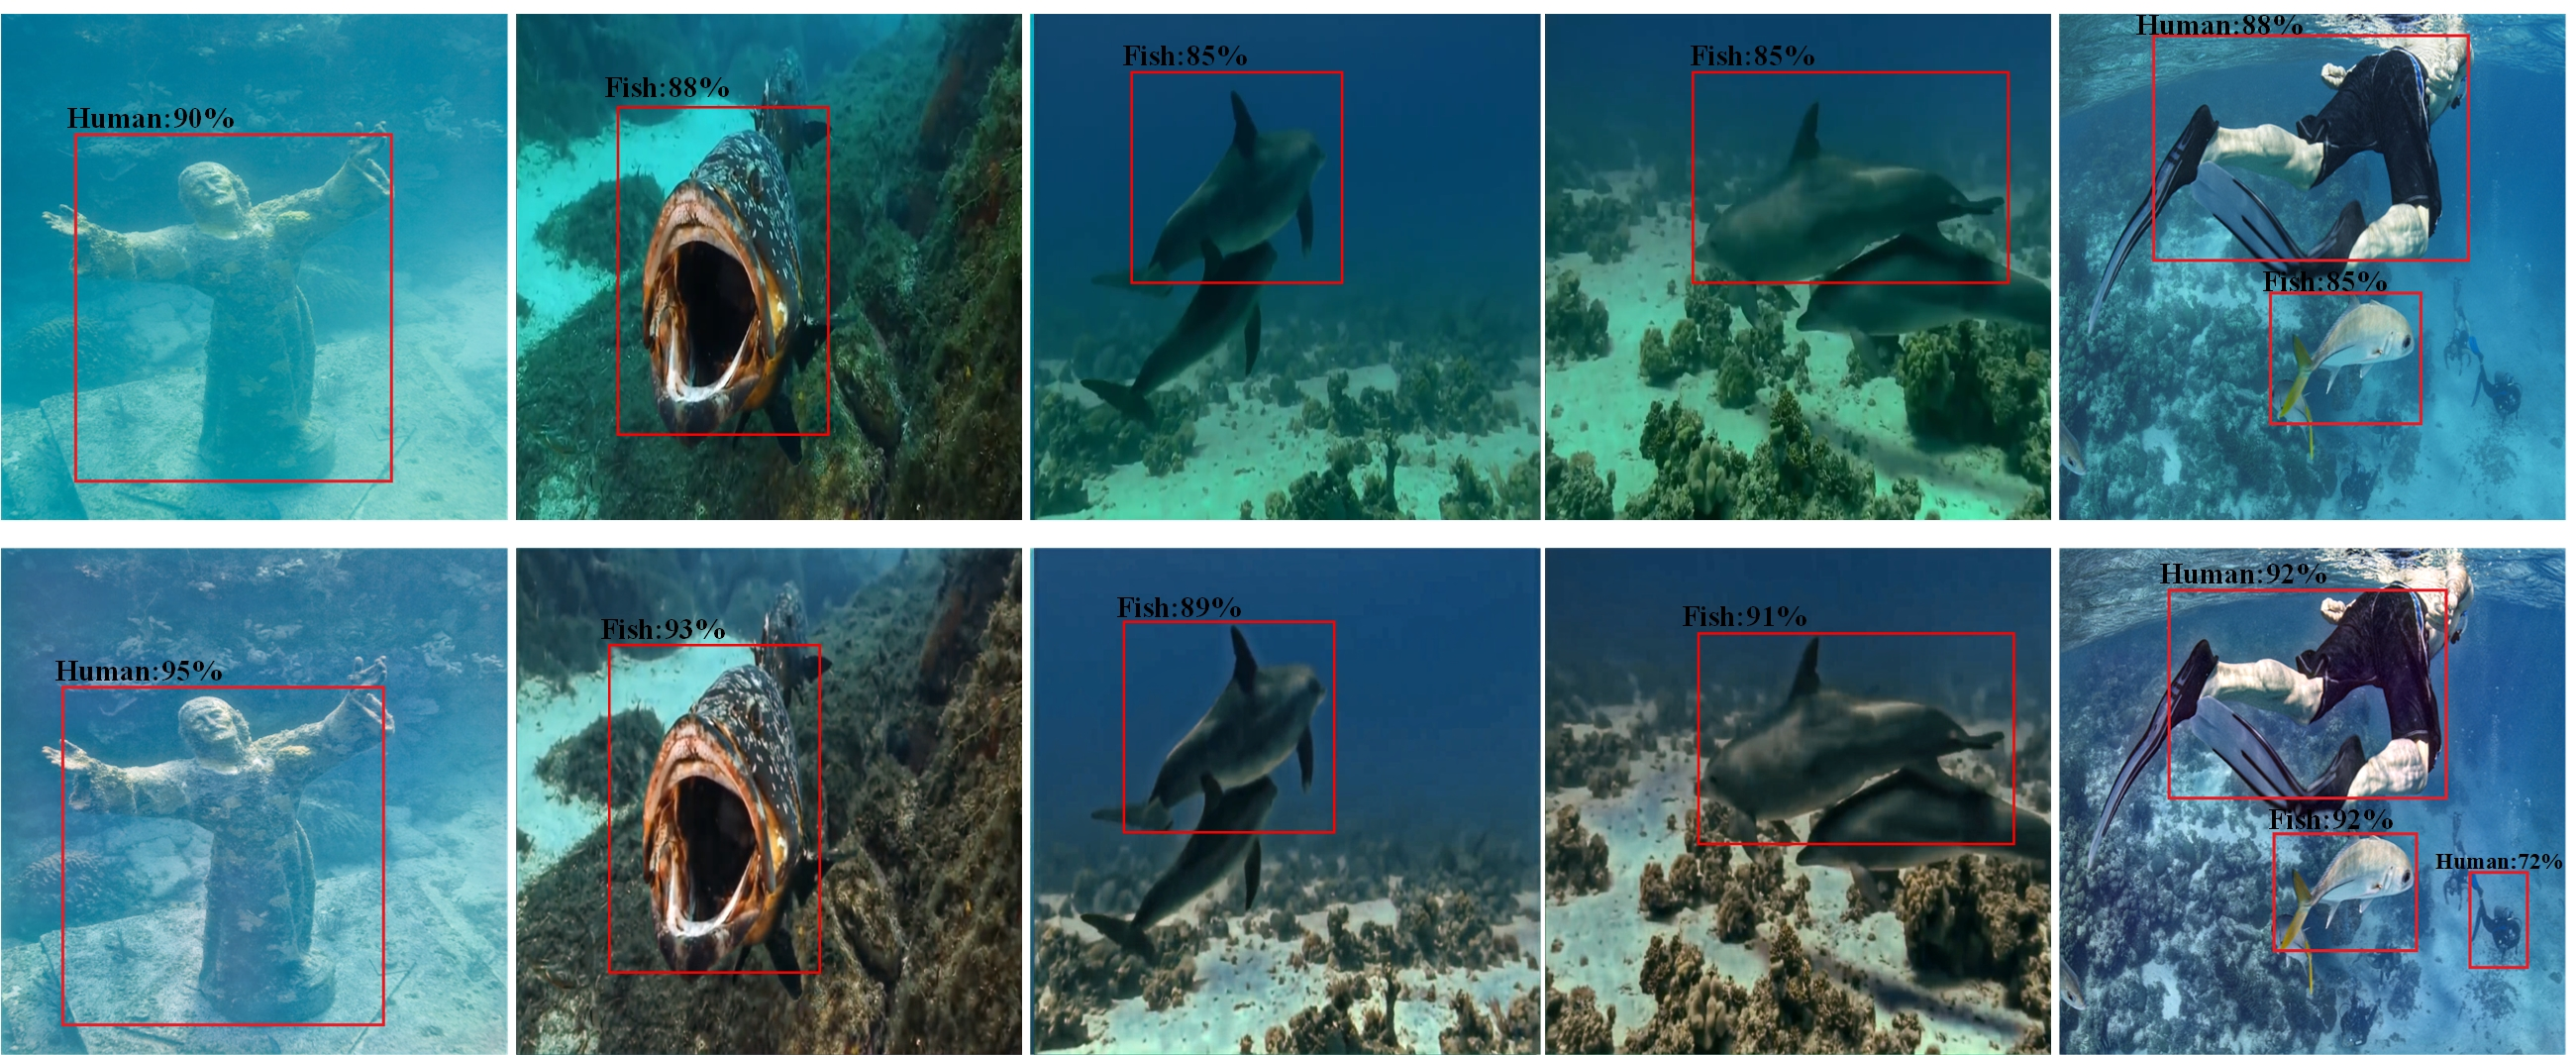
\includegraphics[width=0.7\textwidth]{Figs/Fig10.jpg}

}
\caption{The improvement of object recognition before (the top row) and after (the bottom row) LCNet-based UIE.}
\label{Fig10}
\end{figure*}




\begin{figure*}[ht]
\centering  %图片全局居中
\subfigure[]
{
\label{Fig11-1}
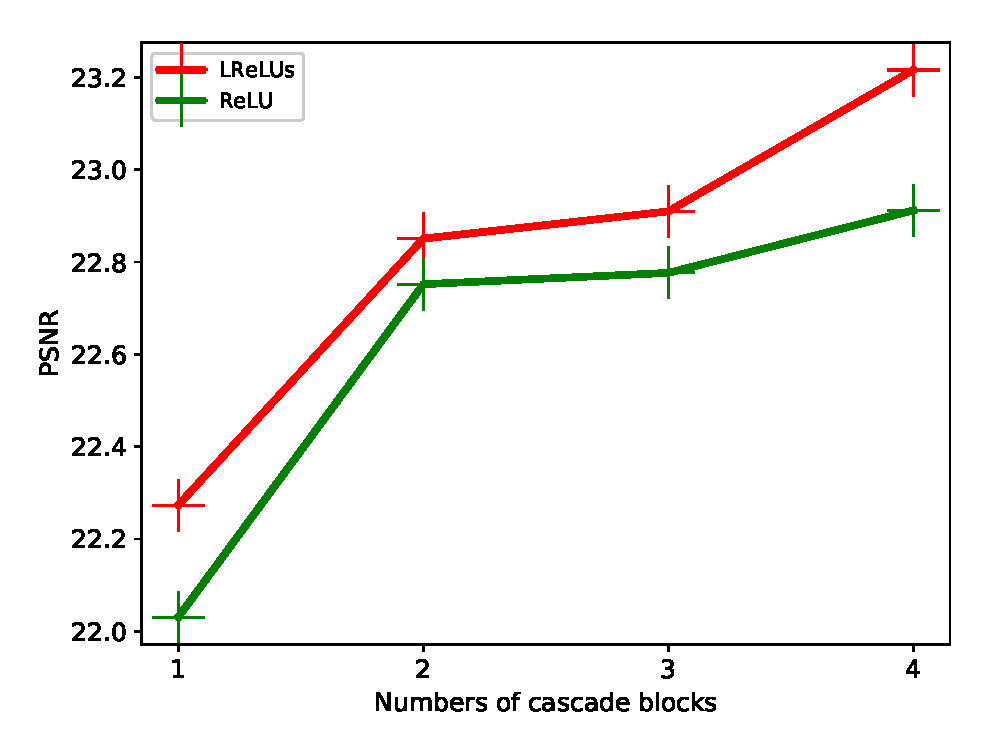
\includegraphics[width=6cm,height=5.5cm]{Figs/Fig11-1.eps}
}\hspace{12mm}
\subfigure[]{
\label{Fig11-2}
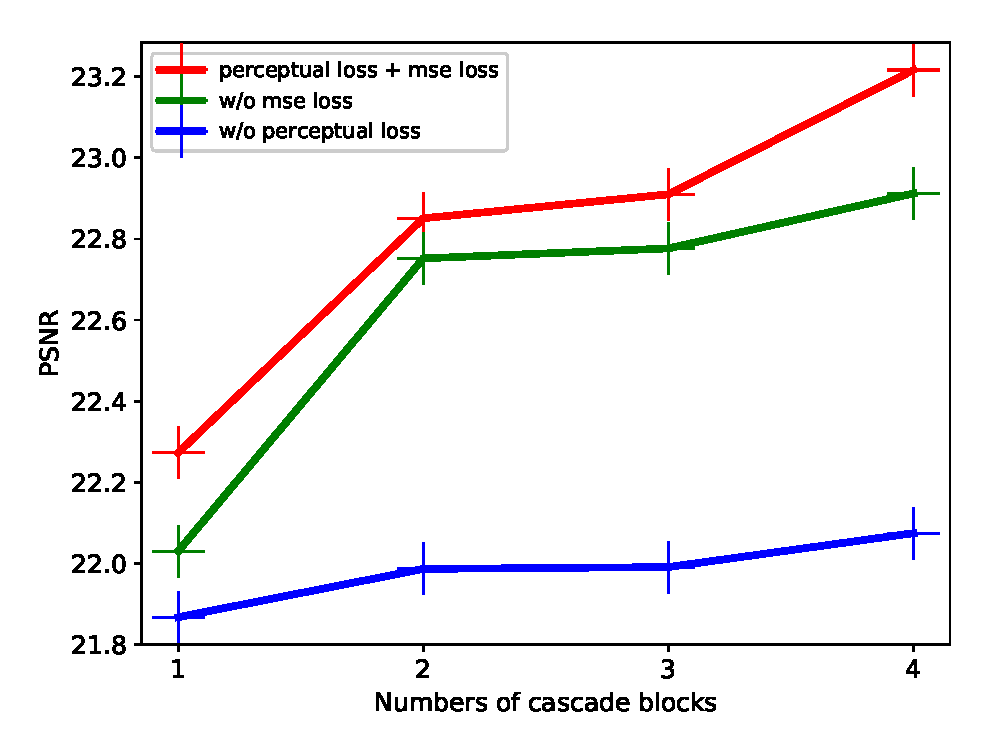
\includegraphics[width=6cm,height=5.5cm]{Figs/Fig11-2.eps}}
\caption{Comparisons of our method using  different (a) activation functions and (b) loss functions.}
\label{Fig11}
\end{figure*}


\begin{figure}[htbp] 
	\centering  %图片全局居中  
	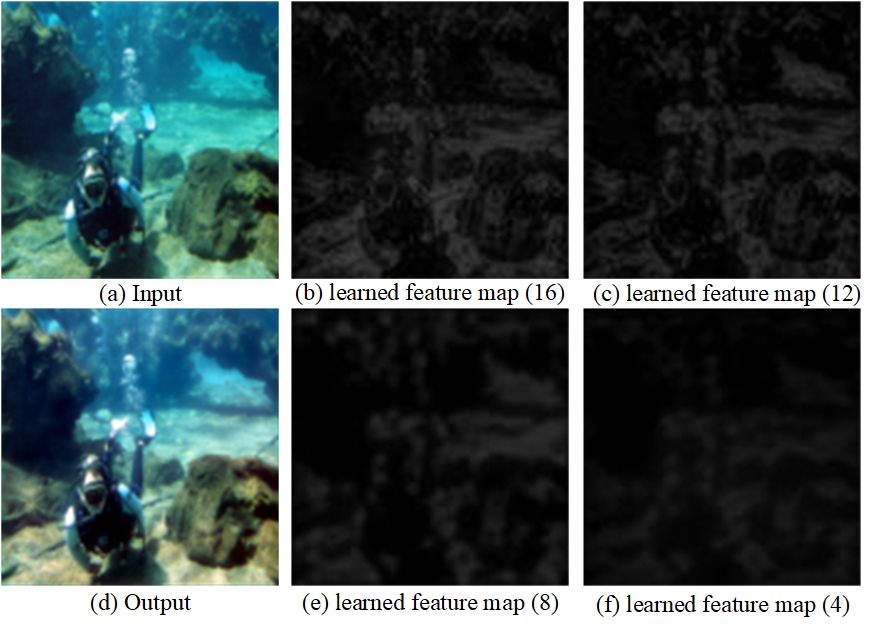
\includegraphics[width=0.45\textwidth]{Figs/Fig12.jpg}
	\caption{Comparisons of different numbers of feature maps.}
	\label{Fig12}
\end{figure}






\subsection{Results on Quantitative Evaluation}
To compare the performances of all methods, we perform both quantitative and qualitative evaluations on each dataset.

First of all, we compare all methods on the synthetic dataset and the UIEB dataset (except its challenging set), where the reference images are available for full reference quality evaluation. Four full-reference quality metrics are utilized: Peak Signal to Noise Ratio (PSNR), Structural SIMilarity (SSIM), Mean Squared Error (MSE) and Learned Perceptual Image Patch Similarity (LPIPS) \cite{zhang2018perceptual}. Among them, the PSNR and SSIM evaluate the image similarity, where a higher score indicates a better performance, and the other two metrics evaluate the discrepancy, which favors lower scores. All comparison results are summarized in Tables \ref{tab1}, \ref{tab2}, \ref{tab3}. Due to the space limit, we provide the average scores of all methods only. The values colored in red and blue indicate the best and second-best results, respectively. As can be observed, the proposed LCNet outperforms the compared methods in most cases. Even in some cases for which our models are not the best or second-best, its performances are still close to the best results in most of quality metrics.

We also compare all methods in the challenging set of UIEB and the SQUID dataset, where the reference images are unavailable. In such case, we utilize the non-reference quality metrics including Underwater Color Image Quality Evaluation (UCIQE) \cite{yang2015underwater}, Underwater Image Quality Measure (UIQM) \cite{panetta2015human},  Cross Correlation Function (CCF) \cite{CCF} and Integrated Local Natural Image Quality Evaluator (ILNIQE) \cite{LNIQE}. All of them give higher scores for higher quality images. The comparison results in UIEB challenging set and SQUID are shown in Tables \ref{tab4} and \ref{tab5}, respectively. They show that our model achieves the best or second-best scores in three of the four quality metrics. To the best of our knowledge, there is no metric with overwhelming superiority in the state-of-the-art UIE quality assessment. Therefore, we can still conclude that our LCNet outperforms the other models for its superior performances in most quality metrics.

In addition, we conduct the runtime analysis to examine the time efficiency of our lightweight model. As shown in Table \ref{tab6}, LCNet achieves the fastest computation. Compared with the fastest state-of-the-art, our model achieves a significant run-time reduction of 55.3\(\%\) on average. This fact indicates that our model achieves both quality improvement and complexity reduction. Moreover, Table \ref{tab6} also shows that, compared with deep learning-based state-of-the-arts, our model significantly reduces the number of model parameters and the number of FLOPs (Floating Point Operations), which also demonstrates the efficiency of our model.



\subsection{Results on Qualitative Evaluation}
 Fig. \ref{Fig5} shows the results of some synthetic samples.
 The compared algorithm might generate images with unnatural
colors or low contrasts. For example, UDCP \cite{UDCP} produces distinctly darkish results, ODM \cite{Histogram-prior} causes over-enhancement, UIBLA \cite{blurriness-based} introduces color deviations and LPNet \cite{fu2019lightweight} tends to generate obvious blurring artifacts. In contrast, our method generates visually pleasant results across all degradation types, showing more consistent color, with fewer effects of vignetting and attenuation compared to the other methods. 
 
The visual comparisons of various methods on the UIEB are also illustrated Figs. \ref{Fig6}, \ref{Fig7}. To better represent the diversity of underwater scenarios, we intentionally select images with different types. From the results, Fusion-Based \cite{fusion-based} and GDCP \cite{GDCP} introduce reddish or greenish colors, LPNet \cite{fu2019lightweight} still tends to leave some blurry parts of UIE images, UIBLA \cite{blurriness-based} overly sharpens the images, and Dense-GAN \cite{dense-gan} causes over-enhancement and over-saturation. Water-CycleGAN \cite{water-gan} produces color casts because it tends to translate content and structure of images to the underwater images. As for evaluations on SQUID \cite{berman2020underwater}, Fig. \ref{Fig8} shows that Ancuti \textit{et al.} (2017) \cite{ancuti2017color} produces distinctly darkish results, while UIBLA \cite{blurriness-based} and Berman \textit{et al.} \cite{berman2020underwater} introduce artificial colors or color deviations. In contrast, our method leads to more consistent colors across various views. It can also reduce vignetting and attenuation effects while better preserving the structures of individual objects in underwater images.

The proposed LCNet also benefits downstream object recognition under underwater environment, which can be demonstrated by a comparison study. First, we generally collect 150 UIEB images with detected objects: 65 with humans (\textit{e.g.} divers) and 85 with fishes, and then enhance them with our LCNet. Second, we pretrain a YOLOv4 \cite{bochkovskiy2020yolov4} model with UIEB database \cite{water-net} for underwater object recognition. Third, we compare the performances of object detection with the original and enhanced images. Fig. \ref{Fig9} shows the different recognition confidence distributions of the two groups of images. It can be easily concluded that our enhancement leads to an improvement of object recognition. Such improvement can also be demonstrated by the results in Fig. \ref{Fig10}, where all recognition confidences are improved. In particular, an extra diver is successfully detected after LCNet-based UIE.



%In Table \ref{tableo1}, the average confidence scores of human and fish images can be improved 6.1 \(\%\) and 7.1 \(\%\), respectively. Meanwhile, in Tables \ref{tableo2} and \ref{tableo3}, the variation of confidence scores can be decreased significantly. These experiments clearly demonstrate our LCNet-based UIE task could help significantly improve the downstream computer vision tasks for underwater images.
% \begin{table}[htbp]
%\caption{Average confidence score \(\%\) of object detetcion.}
%\centering
%\begin{tabular}{|c|c|c|} 
%\hline
%Methods&Original Image&Enhanced Image\\
%\hline
%Average Confidence Score (\(\%\)) &87.2\(\%\) &93.8\(\%\)  \\
%\hline 
%\end{tabular}
%\label{tableo} 
%\end{table}



%
% \begin{table}[htbp]
%\caption{Average confidence scores \(\%\) of human and fish images.}
%\centering
%\begin{tabular}{|c|c|c|} 
%\hline
%Input& Human & Fish \\
%\hline
%Average Confidence Score (\(\%\)) (Original Image) &88.7\(\%\) &86.0\(\%\)\\
%\hline
%Average Confidence Score (\(\%\)) (Enhanced Image) &94.8\(\%\)&93.1\(\%\)\\
%\hline
%\end{tabular}
%\label{tableo1} 
%\end{table}


% \begin{table}[htbp]
%\caption{Variation of confidence scores of all images.}
%\centering
%\begin{tabular}{|c|c|c|} 
%\hline
%Input&Original Image&Enhanced Image\\
%\hline
%Variation &4.213 &1.956  \\
%\hline 
%\end{tabular}
%\label{tableo2} 
%\end{table}


% \begin{table}[htbp]
%\caption{Variation of confidence scores of human and fish images.}
%\centering
%\begin{tabular}{|c|c|c|} 
%\hline
%Input& Human & Fish \\
%\hline
%Variation of Confidence Score (Original Image)  &4.395 &4.033\\
%\hline
%Variation of Confidence Score (Enhanced Image) &2.223&1.640\\
%\hline
%\end{tabular}
%\label{tableo3} 
%\end{table}




\subsection{Ablation Study}
To further examine the effectiveness of our framework, we investigate the different configurations and study their impacts on performance.


\subsubsection{Number of Pyramid Levels}

In our model, we utilize \(N\) to denote the number of pyramid levels and cascaded sub-networks. Generally speaking, a larger number will benefit model performance while leading to an inevitably increase of parameters. According to \cite{lai2018fast}, a typical number of \(N\) should range from 3 to 5. In Table \ref{tab7}, we present the performances of our model with different \(N\) values. It can be seen that \(N\) = 4 and \(N\) = 5 achieve similar performance in terms of PSNR and SSIM, while \(N\) = 4 leads to greatly reduced parameters. Therefore, we select \(N\) = 4 in our work.


\subsubsection{Number of Recursive Blocks}

In each pyramid level, we design a set of cascaded sub-networks. The UIEB test results in Fig. \ref{Fig11} show performance improvement with an increased number of blocks. It also demonstrates the superiority of LReLUs as the activate function in Fig. \ref{Fig11}-(a). If the application scenario changes, one can detach a portion of our model to meet varying computational requirements at test. For instance, we can simplify our model by using two cascade blocks (namely LCNet-2), which are still able to achieve an average PSNR of 22.85dB on UIEB. This performance still outperforms some popular algorithms. Meanwhile, as shown in Table \ref{tab8}, its number of parameters is greatly reduced by 54.6\(\%\) (from 23,325 to 10,593). This demonstrates the flexibility of our model to offer different trade-offs between quality and complexity different scenarios.


\begin{table}[ht]
\centering
\caption{PSNR and SSIM comparisons on UIEB for different numbers of pyramid levels.}
\setlength{\tabcolsep}{4mm}{
\begin{tabular}{|c|c|c|c|} %l(left)居左显示 r(right)居右显示 c居中显示
\hline 
Pyramid levels&\(N = 3\) &\(N = 4\) &\(N = 5\) \\
\hline  
PSNR&22.69&\textbf{23.22}&23.43\\
\hline 
SSIM&0.897&\textbf{0.923}&0.926\\
\hline
Parameters&10,140&\textbf{23,325}&60,390\\
\hline
\end{tabular}}
\label{tab7}
\end{table}

\begin{table}[h]
\centering
\caption{Comparison of complexity in terms of model parameters.}
\setlength{\tabcolsep}{0.6mm}{
\begin{tabular}{|c|c|c|c|c|c|} %l(left)居左显示 r(right)居右显示 c居中显示
\hline 
Methods&Water-Net \cite{water-net}&UWCNN \cite{uwcnn}&LCNet-2&LCNet-3&LCNet-4(ours)\\
%\hline  
%PSNR&19.113&20.048&22.851&22.905&\textbf{23.216}\\
%\hline 
%SSIM&0.7971&0.7761&0.9085&0.9174&\textbf{0.9229}\\
\hline
Parameters&1,090,668&90,646&\textbf{10,593}&16,392&23,325\\
\hline
\end{tabular}
}

\label{tab8}
\end{table}

\subsubsection{Loss Function}
To validate the effectiveness of our loss function, we train the LCNet model with MSE and perceptual loss only and compare their performances with our complete model. Fig. \ref{Fig11}-(b) indicates that each component has its own performance contribution, which justifies the overall design. Moreover, we also conduct experiments to evaluate the impact of \(\lambda\). Although \(\lambda\) = 0.02 is a popular setting, some works also use \(\lambda\) values of 0.01 and 0.04 \cite{dehazeli2018single,zhou2019spatio}. In Table \ref{tab9}, the experiment demonstrates the superior performance of \(\lambda\) = 0.02 in our model.

\begin{table}[ht]
\centering
\caption{PSNR and SSIM comparisons on UIEB for different values of \(\lambda\).}
\setlength{\tabcolsep}{4mm}{
\begin{tabular}{|c|c|c|c|} 
\hline 
Values&\(\lambda\) = 0.01 &\(\lambda\) = 0.02  &\(\lambda\) = 0.04  \\
\hline  
PSNR&23.02&\textbf{23.22}&23.15\\
\hline 
SSIM&0.901&\textbf{0.923}&0.912\\
\hline
\end{tabular}}
\label{tab9} 
\end{table}



\begin{table}[h]
\centering
\caption{PSNR and SSIM comparisons on UIEB for different numbers of feature maps.}
\begin{tabular}{|c|c|c|c|c|} %l(left)居左显示 r(right)居右显示 c居中显示
\hline 
Number of feature maps&16&12&8&4\\
\hline  
PSNR&\textbf{23.22}&23.14&22.81&21.99\\
\hline 
SSIM&\textbf{0.923}&0.923&0.895&0.854\\
\hline
\end{tabular}
\label{tab10}
\end{table}





\subsubsection{Number of Learned Feature Maps}
We also conduct an experiment on UIEB with an increased number of feature maps (out of total 16 feature maps for all convolutional layers of each sub-network). Fig. \ref{Fig12} visualizes four learned feature maps generated by a sub-network, where each learned feature map enhances a certain aspect of a given image. For instance, the learned representation with 16 feature maps highlights specific textures, which is not evidently shown in the input image. Besides, the quantitative results in Table \ref{tab10} show the performance gain achieved by the diversity of learned features. These experiments demonstrate that effectiveness of feature maps that more feature maps improve the performance of UIE modeling. 






\section{Conclusions}
In this paper, we proposed a lightweight deep network for UIE. The proposed LCNet consists of three steps: Laplacian pyramid-based image decomposition, sub-network-based multi-scale enhancement and reconstruction of enhanced images. Specifically, we employ cascaded sub-networks to predict sub-band residuals in a coarse-to-fine fashion to extract a diversity of features. In addition, to develop a lightweight model, we introduce the recursive strategy for model and parameter reuse. Experimental results demonstrate the effectiveness, robustness and low complexity of our UIE model.
\bibliography{refs}


\begin{IEEEbiography}[{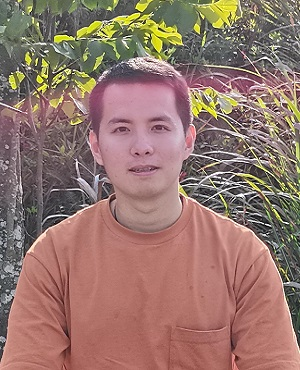
\includegraphics[width=1.25in,height=1.25in,clip,keepaspectratio]{biography/n_jiang.jpg}}]{Nanfeng Jiang} received the B.S. and M.S. degrees in computer science from Fujian Normal University, Fuzhou, China, in 2016 and 2019, respectively. He is currently pursuing the Ph.D. degree with the College of Physics and Information Engineering, Fuzhou University, China. His current research interests include image/video enhancement, and computer vision.
\end{IEEEbiography}
\vspace{-2 mm} 
\begin{IEEEbiography}[{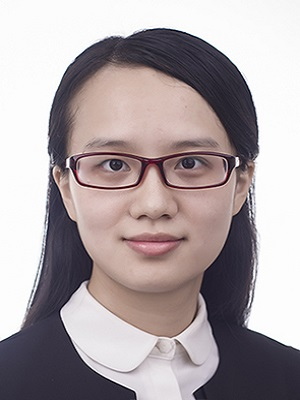
\includegraphics[width=1.25in,height=1.25in,clip,keepaspectratio]{biography/w_chen.jpg}}]{Weiling Chen} (Member, IEEE) received the B.S. and Ph.D. degrees in communication engineering from Xiamen University, Xiamen, China, in 2013 and 2018, respectively. She is currently a Lecturer with the College of Physics and Information Engineering, Fuzhou University, China. From Sep. 2016 to Dec. 2016, she was visiting at the School of Computer Science and Engineering, Nanyang Technological University, Singapore. Her current research interests include image quality perception, computer vision and underwater acoustic transmission.
\end{IEEEbiography}
\vspace{-2 mm} 
\begin{IEEEbiography}[{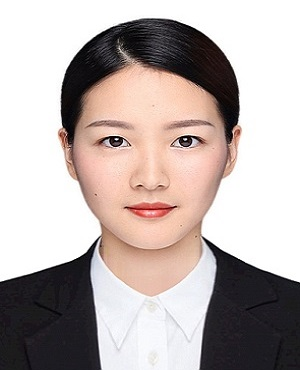
\includegraphics[width=1.25in,height=1.25in,clip,keepaspectratio]{biography/y_lin.jpg}}]{Yuting Lin} received the B.S. degree in communication engineering from Southwest University, Chongqing, China, in 2018, and the M.S. degree in communication and information system from Fuzhou University, Fuzhou, China, in 2021.
Her research interests include image processing and quality perception.
\end{IEEEbiography}
\vspace{-2 mm} 
\begin{IEEEbiography}[{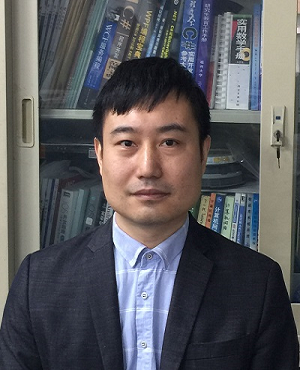
\includegraphics[width=1.25in,height=1.25in,clip,keepaspectratio]{biography/t_zhao.png}}]{Tiesong Zhao} (Senior member, IEEE) received the B.S. degree in electrical engineering from the University of Science and Technology of China, Hefei, China, in 2006, and the Ph.D. degree in computer science from the City University of Hong Kong, Hong Kong, in 2011.
He served as a Research Associate with the Department of Computer Science, City University of Hong Kong (2011-2012), a Postdoctoral Fellow with the Department of Electrical and Computer Engineering, University of Waterloo (2012-2013) and a Research Scientist with the Ubiquitous Multimedia Laboratory, The State University of New York at Buffalo (2014-2015).

He is currently a Minjiang Distinguished Professor in the College of Physics and Information Engineering, Fuzhou University, China.
His research interests include multimedia signal processing, coding, quality assessment and transmission. Due to his contributions in video coding and transmission, he received the Fujian Science and Technology Award for Young Scholars in 2017. He has also been serving as an Associate Editor of IET Electronics Letters since 2019.
\end{IEEEbiography}
\vspace{-2 mm} 
\begin{IEEEbiography}[{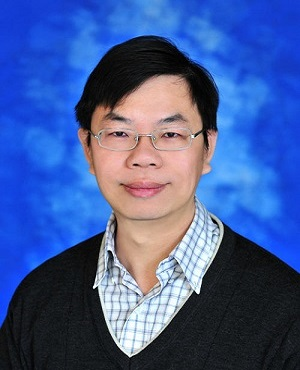
\includegraphics[width=1.25in,height=1.25in,clip,keepaspectratio]{biography/cw_lin.jpg}}]{Chia-Wen Lin} (Fellow, IEEE) received the Ph.D. degree in electrical engineering from National Tsing Hua University (NTHU), Hsinchu, Taiwan, in 2000. He was with the Department of Computer Science and Information Engineering, National Chung Cheng University, Taiwan, from 2000 to 2007. Prior to joining academia, he worked for the Information and Communications Research Laboratories, Industrial Technology Research Institute, Hsinchu, Taiwan, from 1992 to 2000. He is currently a Professor with the Department of Electrical Engineering and the Institute of Communications Engineering, NTHU. He is also the Deputy Director of the AI Research Center, NTHU. His research interests include image and video processing, computer vision, and video networking.

Dr. Lin was a Steering Committee member of the IEEE Transactions on Multimedia from 2014 to 2015. He was a Distinguished Lecturer of the IEEE Circuits and Systems Society from 2018 to 2019. He has also served as the President of the Chinese Image Processing and Pattern Recognition Association, Taiwan, from 2010 to 2019. His papers won the Best Paper Award of IEEE VCIP 2015, Top 10\% Paper Awards of IEEE MMSP 2013, and the Young Investigator Award of VCIP 2005. He received the Young Investigator Award presented by Ministry of Science and Technology, Taiwan, in 2006. He was the Chair of the Multimedia Systems and Applications Technical Committee of the IEEE Circuits and Systems Society from 2013 to 2015. He has served as the Technical Program Co-Chair of IEEE ICME 2010. He will be the General Co-Chair of IEEE VCIP 2018 and Technical Program Co-Chair of IEEE ICIP 2019. He has served as an Associate Editor for the IEEE Transactions on Image Processing, the IEEE Transactions on Circuits and Systems for Video Technology, the IEEE Transactions on Multimedia, the IEEE Multimedia, and the Journal of Visual Communication and Image Representation.
\end{IEEEbiography}




% that's all folks
\end{document}


